\documentclass[oneside]{report}
\usepackage[table]{xcolor}
\usepackage[utf8]{inputenc}
\usepackage[utf8]{vietnam}
\usepackage{graphicx}
\usepackage{nameref}
\usepackage{multicol}
\usepackage{tikz}
\usepackage{rotating}
\usepackage{bbding}
\usepackage{latexsym}
\usepackage{pifont}
\usepackage{pgf-pie}
\usepackage{pgfplots}
\usepackage[nottoc]{tocbibind}
\usepackage{makecell}
\usepackage{tipa}
\usepackage{nicematrix}
\usepackage{acro}
\acsetup{use-id-as-short}

\usepackage[ruled,vlined]{algorithm2e}

% \DeclareAcronym{et}{
%   short=\textbf{ET},
%   long=Eye tracking,
% }

% \DeclareAcronym{pccr}{
%   short=\textbf{PCCR},
%   long= Pupil Center Corneal Reflection,
% }

% \DeclareAcronym{aoi}{
%   short=\textbf{AOI},
%   long=Area of Interest,
% }

% \DeclareAcronym{ocr}{
%   short=\textbf{OCR},
%   long=Optical character recognition,
% }

% \DeclareAcronym{gmm}{
%   short=\textbf{GMM},
%   long=Gaussian Mixture Model,
% }

% \DeclareAcronym{iq}{
%   short=\textbf{IQ},
%   long=Intelligence quotient,
% }

% \DeclareAcronym{lvt}{
%   short=\textbf{LVT},
%   long=Left visual thalamus,
% }

% \DeclareAcronym{idt}{
%   short=\textbf{I-DT},
%   long=Dispersion-Threshold Identification,
% }

% \DeclareAcronym{ivt}{
%   short=\textbf{I-VT},
%   long=Velocity-Threshold Identification,
% }

\NewAcroTemplate[list]{customtable}
  {
    \acronymsmapF
      { \AcroAddRow{\acrowrite {short}&\acrowrite {list}\\} }
      { \AcroRerun }  
    \acroheading
    \acropreamble
    \par \noindent
    \begin{NiceTabularX}{\linewidth}{lX}[hvlines, cell-space-limits=3pt]
      \AcronymTable
    \end{NiceTabularX}
  }


\makeatletter
\newcommand{\unchapter}[1]{%
  \begingroup
  \let\@makechapterhead\@gobble % make \@makechapterhead do nothing
  \chapter{#1}
  \endgroup
}
\makeatother

\hyphenpenalty=5000
\tolerance=500

% % Diagram setting
% \usepackage{tikz}

% set font, font size and spacing
\usepackage{times}
\usepackage{scrextend}
\changefontsizes{13pt}
\renewcommand{\baselinestretch}{1.3}
% section spacing
\usepackage{titlesec}
\titlespacing*{\section}{0pt}{0.5\baselineskip}{0.2\baselineskip}
\titlespacing*{\subsection}{0pt}{0.4\baselineskip}{0.2\baselineskip}

% setup page layout
\usepackage[a4paper,left=30mm,top=25mm,bottom=30mm,right=20mm,]{geometry}

% Acronyms Auto
\usepackage[nopostdot,toc,acronym,nomain,nonumberlist]{glossaries}
\makeglossaries
\setacronymstyle{long-short}
% \loadglsentries[acronym]{FrontMatter/Acronyms}
\setlength{\glsdescwidth}{0.7\linewidth}

% % prevent text overflow
% \usepackage{babel}
% \newcommand\fh{\babelhyphen{hard}}

% Change indent
% \usepackage{indentfirst} % indent also after section titles
\setlength{\parindent}{1cm}
\usepackage{enumitem}
\setlist{leftmargin=1cm}

% paragraph spacing
\setlength{\parskip}{0.5em}

% Change enumerate label
\usepackage{enumitem}

% Page numbering at the center top of page
% \usepackage{fancyhdr} % Custom headers and footers
% \pagestyle{fancyplain} % Makes all pages in the document conform to the custom headers and footers
% \fancyhead[L]{}% Empty left header
% \fancyhead[C]{\thepage} % Page numbering for center header  
% \fancyhead[R]{}% Empty right header
% \fancyfoot[L]{}% Empty left footer
% \fancyfoot[C]{}% Empty center footer
% \fancyfoot[R]{}% Empty left footer

% natbib
% if use natbib, please comment out the cite
\usepackage[sort,numbers]{natbib}
% Citation
% \usepackage{cite}

% Math equation
\usepackage{amssymb}
\usepackage{amsmath}

% Table
\usepackage{multirow}
\usepackage{longtable}
\usepackage{bigstrut}

% Cover
\usepackage{pdfpages}

% Subfigure
\usepackage[labelsep=period]{caption}
\usepackage{subcaption}

% pstricks fig
\usepackage{epsfig}

% Table of Contents
\usepackage[hidelinks]{hyperref}
% \usepackage[unicode]{hyperref}
% Uncomment if you want leading dot for chapter
\usepackage{tocloft}
\renewcommand{\cftpartleader}{\cftdotfill{\cftdotsep}} % for parts
\renewcommand{\cftchapleader}{\cftdotfill{\cftdotsep}} % for chapters

% table fixed width column
\usepackage{array}
\newcolumntype{L}[1]{>{\raggedright\let\newline\\\arraybackslash\hspace{0pt}}m{#1}}
\newcolumntype{C}[1]{>{\centering\let\newline\\\arraybackslash\hspace{0pt}}m{#1}}
\newcolumntype{R}[1]{>{\raggedleft\let\newline\\\arraybackslash\hspace{0pt}}m{#1}}

% define function and variable
\def\highlight#1{\texttt{\textbf{#1}}}


\hyphenation{Nan-yang}


\begin{document}
%---------------------------------------------
% Front Matter
%---------------------------------------------
% \includepdf[pages=-, fitpaper=true]{FrontMatter/cover.pdf}
\begin{titlepage}
    \begin{tikzpicture}[remember picture,overlay,inner sep=0,outer sep=0]
    \draw[line width=4pt] ([xshift=-1.5cm,yshift=-2cm]current page.north east) coordinate (A)--([xshift=2.5cm,yshift=-2cm]current page.north west) coordinate(B)--([xshift=2.5cm,yshift=2cm]current page.south west) coordinate (C)--([xshift=-1.5cm,yshift=2cm]current page.south east) coordinate(D)--cycle;
   \end{tikzpicture}
    \begin{center}
    % {\large\bfseries Bản nháp - \today \par}
    % \vspace{1cm}
    {\normalsize\textbf{ĐẠI HỌC QUỐC GIA HÀ NỘI}\par}
    {\normalsize\textbf{TRƯỜNG ĐẠI HỌC CÔNG NGHỆ}\par}
    \vspace{1cm}
    
    \begin{figure}[h!]
        
\includegraphics[width=0.25\textwidth]{FrontMatter/uet-logo.png}
        \centering
    \end{figure}
    
    {\large\bfseries Nguyễn Văn Quân \par}
    
    %\vspace{3in}
    \vspace{2cm}
    
    {\Large\bfseries
    \begin{minipage}{0.92\textwidth}
        \centering
        TỐI ƯU BỘ QUY TẮC WAF NHẰM\\[0.25em]
        PHÁT HIỆN VÀ NGĂN CHẶN\\[0.25em]
        CÁC KỸ THUẬT TẤN CÔNG LẨN TRÁNH
    \end{minipage}\par}
         
    \vspace{2cm}
    
    {\large\bfseries KHÓA LUẬN TỐT NGHIỆP ĐẠI HỌC HỆ CHÍNH QUY\par}
    {\large\bfseries Ngành: Công nghệ thông tin\par}
        
    \vspace{1.5cm}
    
    \vfill

    

    {\large\bfseries Hà Nội - \the\year{} \par}
    \end{center}
\end{titlepage}
\thispagestyle{empty}
\begin{center}
    \begin{tikzpicture}[remember picture,overlay,inner sep=0,outer sep=0]
    \draw[line width=4pt] ([xshift=-1.5cm,yshift=-2cm]current page.north east) coordinate (A)--([xshift=2.5cm,yshift=-2cm]current page.north west) coordinate(B)--([xshift=2.5cm,yshift=2cm]current page.south west) coordinate (C)--([xshift=-1.5cm,yshift=2cm]current page.south east) coordinate(D)--cycle;
   \end{tikzpicture}
    
    {\normalsize\textbf{ĐẠI HỌC QUỐC GIA HÀ NỘI}\par}
    {\normalsize\textbf{TRƯỜNG ĐẠI HỌC CÔNG NGHỆ}\par}
    \vspace{2cm}

    {\large\bfseries Nguyễn Văn Quân \par}

    %\vspace{3in}
    \vspace{2cm}

    {\Large\bfseries
    \begin{minipage}{0.92\textwidth}
        \centering
        TỐI ƯU BỘ QUY TẮC WAF NHẰM\\[0.25em]
        PHÁT HIỆN VÀ NGĂN CHẶN\\[0.25em]
        CÁC KỸ THUẬT TẤN CÔNG LẨN TRÁNH
    \end{minipage}\par}
     
    \vspace{2cm}

    {\large\bfseries KHÓA LUẬN TỐT NGHIỆP ĐẠI HỌC HỆ CHÍNH QUY \par}
    {\large\bfseries Ngành: Công nghệ thông tin \par}
    
    \vspace{1.5cm}

    {\large\bfseries {Cán bộ hướng dẫn: \\ThS. Trần Mạnh Cường\\ TS.Nguyễn Thị Thủy}\par}
    % {\large\bfseries Co-Supervisor: Dr. Nguyen Thi Cam Huong\par}
    
    \vspace{1.5cm}

    \vfill
    
    {\large\bfseries Hà Nội - \the\year{} \par}
\end{center} 

\clearpage

\pagenumbering{roman}
\setcounter{page}{1}
\chapter*{Lời cảm ơn}
\addcontentsline{toc}{chapter}{Lời cảm ơn}

Lời đầu tiên, em xin bày tỏ lòng biết ơn chân thành và sâu sắc tới các cán bộ hướng dẫn khóa luận của em, ThS. Trần Mạnh Cường và TS. Nguyễn Thị Thủy. Trong quá trình thực hiện đề tài, các thầy cô đã tận tình định hướng, góp ý về nội dung chuyên môn, phương pháp nghiên cứu và cách trình bày báo cáo, giúp em từng bước hoàn thiện khóa luận này.

Em xin gửi lời cảm ơn tới các thầy cô trong Trường Đại học Công nghệ, Đại học Quốc gia Hà Nội đã giảng dạy, truyền đạt kiến thức nền tảng và tạo điều kiện học tập cho em trong suốt quá trình học tập tại trường. Những kiến thức về công nghệ thông tin, an toàn thông tin, phát triển hệ thống và tư duy nghiên cứu là cơ sở quan trọng để em có thể tiếp cận, triển khai và đánh giá đề tài về Web Application Firewall, ModSecurity và OWASP Core Rule Set.

Em cũng xin cảm ơn gia đình đã luôn yêu thương, động viên và tạo điều kiện tốt nhất để em yên tâm học tập, nghiên cứu. Sự ủng hộ của gia đình là nguồn động lực lớn giúp em vượt qua những khó khăn trong quá trình hoàn thành khóa luận.

Bên cạnh đó, em xin gửi lời cảm ơn tới bạn bè và những người đã đồng hành, chia sẻ tài liệu, trao đổi kiến thức và đóng góp ý kiến trong quá trình em thực hiện đề tài. Những trao đổi này đã giúp em nhìn nhận vấn đề rõ ràng hơn và hoàn thiện hơn các phần nội dung trong khóa luận.

Mặc dù em đã cố gắng thực hiện khóa luận một cách nghiêm túc, đề tài vẫn không tránh khỏi những hạn chế và thiếu sót do giới hạn về thời gian, kinh nghiệm nghiên cứu và phạm vi thực nghiệm. Em rất mong nhận được sự góp ý của các thầy cô và các bạn để khóa luận được hoàn thiện hơn.

\chapter*{Lời cam đoan}
\addcontentsline{toc}{chapter}{Lời cam đoan}


Tôi xin cam đoan đề tài “\textbf{Công nghệ và giải pháp theo dõi chuyển động mắt hỗ trợ trẻ em rối loạn đọc}” được trình bày là do tôi thực hiện. Những gì được viết ra trong khóa luận này không sao chép tài liệu hay sử dụng kết quả nghiên cứu của người khác mà không có trích dẫn cụ thể. Nếu có sai phạm, gian lận, tôi xin chịu hoàn toàn trách nhiệm và nhận bất kỳ hình thức xử phạt nào.

\

\

\begin{table}[h]
\begin{tabular}{p{0.5\textwidth}c}
 & Hà Nội, ngày ... tháng 5 năm 2025 \\
 & \\
 & Sinh viên \\
 &              \\
 &              \\
 &              \\
 & \textbf{Nguyễn Thị Kiều Chinh} 
\end{tabular}
\end{table}
\chapter*{Tóm tắt}
\addcontentsline{toc}{chapter}{Tóm tắt}

\textbf{Tóm tắt:} Web Application Firewall (WAF) là một lớp phòng thủ quan trọng giúp phát hiện và ngăn chặn các request độc hại trước khi chúng tới ứng dụng web. Trong các WAF mã nguồn mở, ModSecurity kết hợp với OWASP Core Rule Set (CRS) là một lựa chọn phổ biến nhờ khả năng phát hiện nhiều nhóm tấn công như Cross-Site Scripting (XSS), SQL Injection (SQLi), Local File Inclusion, Remote Code Execution và các bất thường trong giao thức HTTP. Tuy nhiên, khi CRS được cấu hình ở mức nghiêm ngặt cao, đặc biệt là Paranoia Level 4, số lượng false positives có thể tăng mạnh, dẫn đến việc chặn nhầm traffic hợp lệ và làm giảm khả năng triển khai thực tế của WAF. Bên cạnh đó, các kỹ thuật tấn công hiện đại thường sử dụng encoding nhiều lớp, obfuscation, biến thể cú pháp JavaScript/SQL hoặc payload được thiết kế để né tránh regex, khiến các rule dựa trên liệt kê cố định dễ bị bỏ sót.

Khóa luận này nghiên cứu bài toán tối ưu hóa bộ luật WAF ModSecurity cho phát hiện XSS và SQL Injection bằng phương pháp \textit{Generalized Rules}. Thay vì chỉ liệt kê các payload hoặc từ khóa cụ thể, khóa luận đề xuất cách tiếp cận dựa trên ngữ cảnh và cấu trúc hành vi tấn công. Đối với XSS, hệ thống tập trung vào \textit{execution context}, chẳng hạn thẻ HTML có khả năng thực thi, event handler đi kèm hàm nguy hiểm, protocol URI như \path|javascript:|, DOM sink và các biến thể obfuscation. Đối với SQLi, hệ thống tập trung vào các \textit{semantic patterns} như \path|UNION SELECT|, stacked queries, boolean-based injection, time-based blind SQLi, error-based extraction, out-of-band SQLi, schema enumeration và các kỹ thuật comment/hex encoding.

Giải pháp được hiện thực dưới dạng hai bộ custom rules v2 tích hợp với cơ chế Anomaly Scoring của OWASP CRS. Bộ XSS rules v2 sử dụng dải ID \path|9942xxx| và được tổ chức theo kiến trúc 5 lớp gồm Core XSS, Structural Injection, Encoded/Obfuscated XSS, DOM Context và Advanced Heuristic, kèm một lớp xử lý Base64 riêng. Bộ SQLi rules v2 sử dụng dải ID \path|9943xxx|, phát hiện các nhóm SQLi cổ điển, blind SQLi, error-based/OOB SQLi, advanced encoding và một số heuristic liên quan tới NoSQL hoặc OS-command-via-SQL. Các rule áp dụng chuỗi transform như \path|t:urlDecodeUni|, \path|t:htmlEntityDecode|, \path|t:jsDecode|, \path|t:removeNulls| và \path|t:compressWhitespace| nhằm chuẩn hóa payload trước khi so khớp. Ngoài ra, khóa luận xây dựng cấu hình tuning exclusions để vô hiệu hóa có kiểm soát các CRS rules gây false positive cao hoặc trùng lặp với custom rules v2.

Để đánh giá hiệu quả, khóa luận sử dụng benchmark framework tự động gửi payload tới WAF, phân loại kết quả thành true positives, false negatives, true negatives và false positives, sau đó tính các chỉ số Recall, Precision, False Positive Rate, Accuracy và F1-score. Các tập dữ liệu được sử dụng bao gồm GoTestWAF, Mereani XSS, XSSed-DMOZ và các nguồn dữ liệu HTTP/XSS/SQLi đã được chuẩn hóa. Kết quả thực nghiệm cho thấy hướng generalized rules đặc biệt hiệu quả trong việc giảm false positives trên các tập dữ liệu mixed/benign. Trên Mereani clean, rule gốc đạt recall cao nhưng có FPR khoảng 99.78\%, trong khi custom rules v2 giữ recall khoảng 98.20\% và giảm FPR xuống khoảng 1.05\%. Trên XSSed-DMOZ clean, custom rules v2 đạt recall khoảng 99.71\%, FPR khoảng 0.23\% và accuracy khoảng 99.74\%, trong khi rule gốc có FPR khoảng 99.52\%. Các kết quả này cho thấy việc chỉ tối đa hóa detection rate là chưa đủ; với WAF thực tế, giảm false positives là điều kiện quan trọng để hệ thống có thể được triển khai và vận hành ổn định.

Khóa luận cũng thảo luận minh bạch các giới hạn và đánh đổi của phương pháp. Việc tuning bằng \path|SecRuleRemoveById| giúp giảm đáng kể false positives nhưng cần được phân tích rủi ro, đặc biệt với các CRS rules ngoài phạm vi chính của đề tài như RCE/Shell Injection hoặc các heuristic tổng quát như libinjection SQLi. Hệ thống không tuyên bố thay thế hoàn toàn OWASP CRS hoặc phát hiện 100\% mọi biến thể tấn công mới. Thay vào đó, đóng góp chính của khóa luận là một phương pháp thiết kế rule có cấu trúc, dễ giải thích, có khả năng giảm false positives đáng kể trong phạm vi XSS/SQLi, đồng thời vẫn duy trì recall cao trên các benchmark đã kiểm thử. So với các hướng AI-based detection, WAF rule-based sau tuning có ưu điểm về độ trễ thấp, khả năng giải thích rõ ràng và khả năng cập nhật nhanh bằng cách bổ sung rule mới, phù hợp với yêu cầu triển khai inline trong hệ thống web thực tế.

\vspace{8pt}
\noindent \textit{\textbf{Từ khóa}:} Web Application Firewall, ModSecurity, OWASP CRS, Cross-Site Scripting, SQL Injection, Generalized Rules, Anomaly Scoring, False Positive Reduction.


% Show ToC and change title to Table of Contents
\setcounter{secnumdepth}{3}
\renewcommand{\contentsname}{Mục lục}
\tableofcontents
% \clearpage

% Show list of 
\renewcommand{\listfigurename}{Danh mục hình ảnh}
\listoffigures
\renewcommand{\listtablename}{Danh mục bảng}

\listoftables
\chapter*{Thuật ngữ và từ viết tắt}
\addcontentsline{toc}{chapter}{Thuật ngữ và từ viết tắt}
% \glsaddall

\begin{table}[h]
    \centering
    \renewcommand{\arraystretch}{1.2} % Tăng khoảng cách giữa các hàng
    \begin{tabular}{|C{0.15\textwidth}|C{0.4\textwidth}|C{0.4\textwidth}|}
        \hline
        \textbf{Từ viết tắt} & \textbf{Từ đầy đủ} & \textbf{Ý nghĩa} \\ 
        \hline
        AOI & Area of Interest & Khu vực quan tâm \\ 
        \hline
        OCR & Optical Character Recognition & Nhận dạng ký tự quang học \\
        \hline
        EyeMMV & Eye Movements Metrics \& Visualizations & Thuật toán xử lý số liệu và hình ảnh trực quan chuyển động mắt \\ 
        \hline
        PeyeMMV & Python implementation of EyeMMV & Cài đặt thuật toán EyeMMV bằng Python \\ 
        \hline
        I-VT & Velocity-Threshold Identification & Thuật toán xác định theo ngưỡng vận tốc \\ 
        \hline
        I-DT & Dispersion-Threshold Identification & Thuật toán xác định theo ngưỡng phân tán \\ 
        \hline
    \end{tabular}
    \label{tab:terms}
\end{table}

% \acuseall

\printacronyms[heading=addchap, sort=true, template=customtable]





%--------------------------------------------- 
% Main content
%---------------------------------------------
\renewcommand{\chaptername}{Chương}
\renewcommand{\figurename}{Hình}
\renewcommand{\tablename}{Bảng}
\pagenumbering{arabic}
\setcounter{page}{1}
\chapter{Giới thiệu}
\label{chap:introduction}

Các ứng dụng web hiện nay là nền tảng của thương mại điện tử, dịch vụ công, giáo dục trực tuyến, ngân hàng số và nhiều hệ thống nghiệp vụ. Khi phần lớn dữ liệu và quy trình vận hành được đưa lên môi trường web, lớp ứng dụng trở thành mục tiêu tấn công quan trọng. Trong các rủi ro phổ biến, Cross-Site Scripting (XSS) và SQL Injection (SQLi) vẫn có ảnh hưởng lớn vì chúng khai thác trực tiếp cách ứng dụng xử lý dữ liệu đầu vào của người dùng~\cite{owasp2021top10}. XSS có thể dẫn tới đánh cắp phiên đăng nhập, thực thi mã JavaScript độc hại trên trình duyệt nạn nhân hoặc thay đổi nội dung hiển thị. SQL Injection có thể cho phép kẻ tấn công truy vấn, sửa đổi hoặc phá hoại cơ sở dữ liệu phía sau ứng dụng.

Một hướng phòng thủ phổ biến là triển khai Web Application Firewall (WAF) trước ứng dụng. WAF không thay thế việc lập trình an toàn, nhưng đóng vai trò như một lớp kiểm tra bổ sung: mọi HTTP request đi qua WAF sẽ được phân tích để phát hiện các mẫu tấn công trước khi tới ứng dụng. Trong hệ sinh thái mã nguồn mở, ModSecurity là một WAF engine được sử dụng rộng rãi, còn OWASP Core Rule Set (CRS) là bộ luật phổ biến được triển khai cùng ModSecurity để phát hiện nhiều nhóm tấn công web khác nhau~\cite{modsecurity-crs-overview,owasp-crs-docs}. Tuy nhiên, triển khai WAF hiệu quả không chỉ là bật càng nhiều rule càng tốt. Một hệ thống WAF thực tế cần cân bằng giữa hai mục tiêu: phát hiện được tấn công thật và hạn chế chặn nhầm request hợp lệ.

\section{Bối cảnh an toàn ứng dụng web}
\label{sec:motivation}

Về bản chất, WAF là một cơ chế phòng thủ dựa trên luật. Mỗi request được so khớp với một tập quy tắc mô tả dấu hiệu tấn công. Ví dụ, một request chứa chuỗi \path|<script>alert(1)</script>| có thể bị xem là XSS, hoặc một tham số chứa \path|' OR 1=1--| có thể bị xem là SQL Injection. Nếu chỉ nhìn ở mức trực giác, cách làm này có vẻ đơn giản: càng liệt kê nhiều dấu hiệu nguy hiểm thì WAF càng phát hiện tốt. Tuy nhiên, trong thực tế, cùng một từ khóa hoặc ký tự có thể xuất hiện trong cả ngữ cảnh tấn công và ngữ cảnh hợp lệ. Một website có thể truyền đoạn JavaScript hợp lệ trong tham số, một nội dung hướng dẫn lập trình có thể chứa từ \path|SELECT|, hoặc một form HTML hợp lệ có thể dùng event handler như \path|onsubmit="validate()"|.

Trong bối cảnh nghiên cứu này, vấn đề trọng tâm không phải là xây dựng một WAF hoàn toàn mới, mà là tối ưu bộ luật phát hiện XSS và SQLi trong môi trường ModSecurity/OWASP CRS. Đề tài tập trung vào câu hỏi: làm thế nào để các rule vẫn phát hiện được các kỹ thuật bypass phổ biến, nhưng không chặn nhầm quá nhiều request hợp lệ? Đây là bài toán quan trọng vì false positive cao có thể khiến WAF khó triển khai trong thực tế. Nếu WAF liên tục chặn nhầm người dùng thật, quản trị viên thường buộc phải tắt rule hoặc tăng ngưỡng chặn, từ đó làm giảm hiệu quả bảo vệ.

\section{Thực trạng WAF rule-based và vấn đề nghiên cứu}
\label{sec:problem-overview}

OWASP CRS là một nền tảng quan trọng vì cung cấp sẵn nhiều luật phát hiện tấn công web phổ biến. CRS cũng dùng cơ chế cộng điểm bất thường: mỗi dấu hiệu đáng ngờ làm request tăng điểm, và request chỉ bị chặn khi tổng điểm vượt ngưỡng cấu hình. Cách làm này giúp WAF kết hợp nhiều tín hiệu khác nhau thay vì phụ thuộc vào một rule đơn lẻ. Tuy nhiên, khi cấu hình nghiêm ngặt hơn hoặc bật nhiều rule hơn, WAF thường phát hiện được nhiều dấu hiệu hơn nhưng cũng dễ chặn nhầm request hợp lệ hơn~\cite{owasp-crs-annotated,paranoia-levels-study,waf-benchmark-2024}.

Một hướng cải thiện phổ biến là bổ sung custom rules cho các nhóm tấn công cần ưu tiên, chẳng hạn XSS và SQL Injection. Các nghiên cứu trước cho thấy việc bổ sung rule có thể cải thiện khả năng phát hiện trên benchmark~\cite{researcher-group-2025}. Tuy nhiên, nhiều rule kiểu này vẫn dựa nhiều vào cách liệt kê dấu hiệu đã biết: liệt kê tên hàm JavaScript, tag HTML, từ khóa SQL hoặc một số payload cụ thể. Cách tiếp cận này dễ hiểu và có hiệu quả với các mẫu đã biết, nhưng có ba vấn đề chính ở mức tổng quan.

Thứ nhất, danh sách liệt kê khó bao phủ hết các biến thể tấn công. Kẻ tấn công có thể thay đổi cú pháp, mã hóa payload, chèn khoảng trắng bất thường hoặc dùng cách gọi hàm khác để né rule. Thứ hai, rule quá rộng có thể chặn nhầm dữ liệu hợp lệ, vì người dùng có thể nhập nội dung kỹ thuật chứa HTML, JavaScript hoặc SQL mà không có ý định tấn công. Thứ ba, khi danh sách payload ngày càng dài, rule trở nên khó đọc, khó kiểm thử và khó bảo trì.

Từ thực trạng trên, khóa luận lựa chọn hướng \textbf{generalized rules}: thay vì chỉ hỏi ``request có chứa từ khóa nguy hiểm hay không'', rule cần xét xem dữ liệu đó có nằm trong ngữ cảnh nguy hiểm hay không. Với XSS, trọng tâm là ngữ cảnh có thể thực thi JavaScript. Với SQLi, trọng tâm là cấu trúc có khả năng làm thay đổi ý nghĩa truy vấn. Chương 2 sẽ trình bày chi tiết hơn cơ sở lý thuyết, các phương pháp liên quan và hạn chế của từng hướng; Chương 3 trình bày giải pháp đề xuất dựa trên các phân tích đó.

\section{Mục tiêu nghiên cứu}
\label{sec:objectives}

Mục tiêu tổng quát của khóa luận là \textbf{đánh giá và đề xuất một hướng tối ưu bộ luật WAF ModSecurity cho phát hiện XSS và SQL Injection nhằm giảm false positives, duy trì khả năng phát hiện cao trên các payload tấn công phổ biến, và cải thiện tính bảo trì so với phương pháp enumeration-based}. Mục tiêu này nhấn mạnh kết quả cần đạt được của nghiên cứu, không chỉ dừng ở việc triển khai thêm một tập rule mới.

Các mục tiêu cụ thể bao gồm:

\begin{enumerate}
    \item \textbf{Làm rõ hạn chế của CRS và rule enumeration-based} trong phát hiện XSS/SQLi, đặc biệt về false positives, coverage trước payload biến thể và khả năng bảo trì.

    \item \textbf{Đánh giá khả năng giảm false positives của hướng generalized/context-aware detection}, trong đó rule cần xét ngữ cảnh thực thi hoặc cấu trúc tấn công thay vì bắt từ khóa đơn lẻ.

    \item \textbf{Đánh giá vai trò của decode pipeline} đối với payload encoded/obfuscated, bao gồm URL encoding, HTML entity, JavaScript escape, null byte, whitespace obfuscation và Base64.

    \item \textbf{Đánh giá khả năng mở rộng coverage SQLi} khi sử dụng semantic patterns trên nhiều nhóm kỹ thuật và nhiều hệ quản trị cơ sở dữ liệu, thay vì chỉ bắt một số payload cố định.

    \item \textbf{Đánh giá tác động của tuning exclusions} tới false positive rate và recall trong phạm vi XSS/SQLi, đồng thời ghi nhận các trade-off bảo mật khi vô hiệu hóa một số CRS rules.

    \item \textbf{Phân tích ưu và nhược điểm của WAF rule-based sau tuning} khi đặt cạnh hướng AI-based detection về khả năng giải thích, độ trễ, khả năng cập nhật và tính phù hợp với triển khai real-time.
\end{enumerate}

\section{Câu hỏi nghiên cứu}
\label{sec:research-questions}

Từ mục tiêu trên, khóa luận tập trung trả lời các câu hỏi nghiên cứu sau:

\begin{itemize}
    \item \textbf{RQ1:} Phương pháp generalized/context-aware rules có giúp giảm false positives so với phương pháp enumeration-based trong phát hiện XSS hay không?

    \item \textbf{RQ2:} Việc sử dụng multi-decode pipeline có cải thiện khả năng phát hiện các payload XSS/SQLi được mã hóa hoặc obfuscate hay không?

    \item \textbf{RQ3:} Các SQLi rules dựa trên semantic patterns có mở rộng coverage tốt hơn so với rule chỉ bắt một số payload cố định hay không?

    \item \textbf{RQ4:} Việc tuning CRS bằng cách vô hiệu hóa có chọn lọc các rule gây FP cao có thể giảm false positives mà vẫn giữ recall cao cho XSS/SQLi hay không?

    \item \textbf{RQ5:} Khi so sánh với hướng AI-based detection, WAF rule-based sau tuning có những ưu và nhược điểm gì về khả năng giải thích, độ trễ, khả năng cập nhật và tính phù hợp với triển khai real-time?
\end{itemize}

Các câu hỏi này định hướng cấu trúc của các chương sau. Chương 2 phân tích cơ sở lý thuyết, nghiên cứu liên quan và hạn chế của các phương pháp hiện có; Chương 3 trình bày phương pháp nghiên cứu và giải pháp đề xuất; Chương 4 trình bày thiết kế thực nghiệm và phương pháp đánh giá; Chương 5 trình bày kết quả thực nghiệm; và Chương 6 thảo luận ý nghĩa, giới hạn và trade-off của các kết quả đó.

\section{Phạm vi nghiên cứu}
\label{sec:scope}

Để đảm bảo bài toán đủ tập trung, khóa luận giới hạn phạm vi như sau:

\begin{itemize}
    \item \textbf{Loại tấn công chính:} XSS và SQL Injection. Một số pattern NoSQL hoặc OS-command-via-SQL có thể xuất hiện trong lớp heuristic, nhưng không phải trọng tâm chính.

    \item \textbf{Nền tảng triển khai:} ModSecurity kết hợp OWASP CRS và custom rules. Đề tài không xây dựng WAF engine mới.

    \item \textbf{Dữ liệu đánh giá:} các dataset và benchmark payloads như GoTestWAF, Mereani XSS, XSSed-DMOZ, CSIC 2010 và ECML nếu đã được chuẩn hóa trong pipeline thực nghiệm.

    \item \textbf{Phương pháp đánh giá:} tập trung vào TP, TN, FP, FN và các metrics như Recall, Precision, FPR, Accuracy và F1-score.

    \item \textbf{Tuning:} tập trung vào giảm false positives trong phạm vi XSS/SQLi bằng cách phân tích benchmark và audit logs.
\end{itemize}

Các nội dung ngoài phạm vi gồm: xem RCE/Shell Injection là mục tiêu chính; triển khai production đầy đủ; thay thế toàn bộ OWASP CRS; và cam kết phát hiện mọi zero-day hoặc mọi biến thể tấn công mới. Những giới hạn và rủi ro liên quan tới tuning sẽ được thảo luận chi tiết hơn ở Chương 6.

\section{Đóng góp chính của khóa luận}
\label{sec:contributions}

Khóa luận có các đóng góp chính sau:

\begin{enumerate}
    \item \textbf{Kiến trúc phát hiện XSS context-aware theo nhiều lớp.} Bộ XSS rules v2 sử dụng dải ID \path|9942xxx|, tập trung vào execution context thay vì chỉ bắt từ khóa. Các lớp gồm core XSS, structural injection, encoded/obfuscated payload, DOM context và advanced heuristic.

    \item \textbf{Bộ SQLi rules v2 dựa trên semantic patterns.} Bộ SQLi rules sử dụng dải ID \path|9943xxx|, phát hiện các nhóm kỹ thuật như UNION-based, stacked queries, boolean/time-based blind SQLi, error-based SQLi, OOB SQLi, schema enumeration, comment obfuscation và encoded SQL keywords.

    \item \textbf{Multi-decode pipeline cho payload bị mã hóa.} Giải pháp áp dụng các transform như \path|t:urlDecodeUni|, \path|t:htmlEntityDecode|, \path|t:jsDecode|, \path|t:removeNulls| và \path|t:compressWhitespace|. Ngoài ra, một lớp riêng xử lý Base64 được sử dụng để phát hiện payload sau khi decode.

    \item \textbf{Phương pháp tuning dựa trên dữ liệu.} Khóa luận sử dụng benchmark và audit logs để xác định rule gây FP cao, sau đó phân nhóm rủi ro và cấu hình \path|TUNING-EXCLUSIONS.conf| có kiểm soát.

    \item \textbf{Benchmark framework và đánh giá thực nghiệm.} Hệ thống benchmark tự động gửi payload tới WAF, phân loại TP/TN/FP/FN và sinh báo cáo để so sánh rule gốc, CRS baseline, custom generalized rules v2 và AI model tham chiếu.

    \item \textbf{Phân tích trade-off minh bạch.} Khóa luận không chỉ trình bày kết quả tốt, mà còn thảo luận rủi ro của tuning, đặc biệt là việc vô hiệu hóa một số CRS rules ngoài phạm vi XSS/SQLi như RCE/Shell và trade-off khi tắt libinjection SQLi.
\end{enumerate}

\section{Cấu trúc khóa luận}
\label{sec:thesis-structure}

Phần còn lại của khóa luận gồm năm chương. Chương 2 trình bày cơ sở lý thuyết và các nghiên cứu liên quan. Chương 3 trình bày phương pháp nghiên cứu và giải pháp đề xuất. Chương 4 mô tả thiết kế thực nghiệm và phương pháp đánh giá. Chương 5 trình bày kết quả thực nghiệm và đánh giá. Chương 6 thảo luận các kết quả chính, nêu giới hạn và kết luận khóa luận.

\chapter{Kiến thức liên quan}
\label{chap:related_work}
% -------------------------------------------------------------------
% Introduction of the chapter
% -------------------------------------------------------------------
Để phát triển giải pháp ứng dụng công nghệ theo dõi chuyển động mắt hỗ trợ trẻ rối loạn đọc, chúng ta cần nắm vững kiến thức về rối loạn đọc, các bất thường trong chuyển động mắt của trẻ, cũng như những kiến thức liên quan đến việc ứng dụng công nghệ theo dõi mắt để hỗ trợ nhóm trẻ này. Trong \textbf{Chương 2}, khóa luận sẽ trình bày tổng quan các kiến thức về rối loạn đọc, cũng như những công nghệ liên quan được sử dụng để hoàn thành khóa luận. 
% -------------------------------------------------------------------
% Dyslexia and abnormalities in eye movements
% -------------------------------------------------------------------
\section{Rối loạn đọc và sự khác thường trong chuyển động mắt của người mắc chứng rối loạn đọc}
\label{sec:dysevm}
Rối loạn đọc (Dyslexia) là một hội chứng rối loạn học tập ảnh hưởng đến khả năng đọc chính xác và lưu loát của một cá nhân, được đặc trưng bởi các khó khăn trong nhận diện từ, giải mã từ và đánh vần \cite{roitsch2019overview, american2013diagnostic}. Những người mắc rối loạn đọc thường gặp trở ngại trong việc ánh xạ âm thanh trong ngôn ngữ nói sang ký tự viết, đặc biệt ở các ngôn ngữ có mối quan hệ phức tạp giữa chữ cái và âm thanh chúng biểu thị. Rối loạn đọc không chỉ gây khó khăn trong học tập mà còn có thể dẫn đến các vấn đề tâm lý và xã hội, chẳng hạn như cảm giác thất vọng, tự ti hoặc bị cô lập. Mặc dù có trí thông minh bình thường, trẻ mắc rối loạn đọc thường không đạt được kỹ năng đọc ngang bằng với bạn bè đồng trang lứa, dẫn đến việc bị hiểu lầm là lười biếng hoặc kém thông minh. Hơn nữa, đây là một trong những rối loạn học tập phổ biến nhất, ảnh hưởng từ 5-10\% dân số toàn cầu \cite{khaleghi2022developing}. Do đó, việc chẩn đoán và can thiệp kịp thời cho người mắc rối loạn đọc là rất quan trọng.

Các phương pháp hiện tại để chẩn đoán rối loạn đọc bao gồm kiểm tra kỹ năng đọc, đánh giá ngữ âm, kiểm tra tâm lý, và phỏng vấn phụ huynh cùng giáo viên \cite{lindstrom2019dyslexia}. Tuy nhiên, rối loạn đọc không phải là một căn bệnh mà là một rối loạn phát triển, với biểu hiện khác nhau ở mỗi cá nhân \cite{al2012understanding}. Vì vậy, việc áp dụng cùng một phương pháp chẩn đoán và can thiệp cho tất cả các cá nhân mắc cùng một rối loạn có thể không phản ánh được khó khăn cụ thể của từng người, cũng như không thể đề xuất các biện pháp cá nhân hóa. Bên cạnh các phương pháp đánh giá truyền thống, những cách tiếp cận cho phép quan sát trực tiếp hành vi và chuyển động mắt của từng cá nhân đang ngày càng nhận được sự quan tâm. Nhờ sự phát triển công nghệ, các bài kiểm tra đánh giá đã được số hóa và tích hợp với công nghệ theo dõi chuyển động mắt, mang đến những khả năng mới trong việc chẩn đoán khách quan và chính xác. Phần lớn các nghiên cứu đều cho thấy rằng trẻ rối loạn đọc thường có những đặc điểm chuyển động mắt khác thường so với những trẻ phát triển bình thường khác cùng trang lứa. Nghiên cứu của Jainta và cộng sự tiết lộ rằng người mắc rối loạn đọc kém hơn trong việc kiểm soát song nhãn cầu \cite{jainta2011dyslexic}. Suy giảm thị giác-vận động nhãn cầu ở những người này có thể gây mất ổn định điểm cố định, dẫn đến ảnh hưởng khả năng đọc hiểu. Ngoài ra, trẻ mắc rối loạn đọc thiếu hụt trong quá trình xử lý thông tin, không chỉ đối với văn bản \cite{jones2008elucidating, weiss2022lateralization} mà còn với các kích thích khác như hình ảnh khuôn mặt \cite{galazka2021facial, aasberg2022left}. Sự thiếu hụt này biểu hiện qua dao động liên tục và chuyển động mắt tương đối nhỏ ở trẻ mắc rối loạn đọc so với trẻ phát triển bình thường khi đọc. Đồng thời, trẻ rối loạn đọc cũng có tần suất chuyển động tiến và lùi của nhãn cầu cao hơn đáng kể \cite{pavlidis1985eye}. Những bất thường trong chuyển động mắt này cho thấy tiềm năng lớn của việc ứng dụng công nghệ theo dõi chuyển động mắt để hỗ trợ chẩn đoán và can thiệp rối loạn đọc.


% -------------------------------------------------------------------
% Eye-tracking technology
% -------------------------------------------------------------------
\section{Kiến thức nền tảng}
\label{sec:theoreticalbg}
Bên cạnh những hiểu biết về chứng rối loạn đọc và các bất thường trong chuyển động mắt của người mắc hội chứng này, các kiến thức liên quan đến công nghệ theo dõi chuyển động mắt, nhận diện khu vực quan tâm, nhận dạng ký tự quang học, các đặc trưng chuyển động mắt có giá trị trong việc hỗ trợ trẻ rối loạn đọc, cũng như các phương pháp trực quan hóa, đều đóng vai trò quan trọng trong quá trình ứng dụng công nghệ này để hỗ trợ nhóm đối tượng trên. Trong phần tiếp theo, chúng tôi sẽ trình bày tổng quan những kiến thức có liên quan.

\subsection{Công nghệ theo dõi chuyển động mắt}
\label{subsec:et}
Công nghệ theo dõi chuyển động mắt (Eye tracking) là một phương pháp thu thập và nhận diện chuyển động của mắt khi con người nhìn từ vị trí này sang vị trí khác \cite{poole2006eye}. Theo dõi chuyển động mắt đo lường vị trí và thời điểm ánh mắt hướng tới khi thực hiện một nhiệm vụ hoặc hành động. Công nghệ này xác định mối liên hệ giữa mắt và hệ thần kinh, liên kết chuyển động của mắt với quá trình nhận thức và từ đó đưa ra một cái nhìn sâu rộng vào hoạt động bên trong của não bộ \cite{carter2020best}. 

\begin{figure}[h]
    \centering
    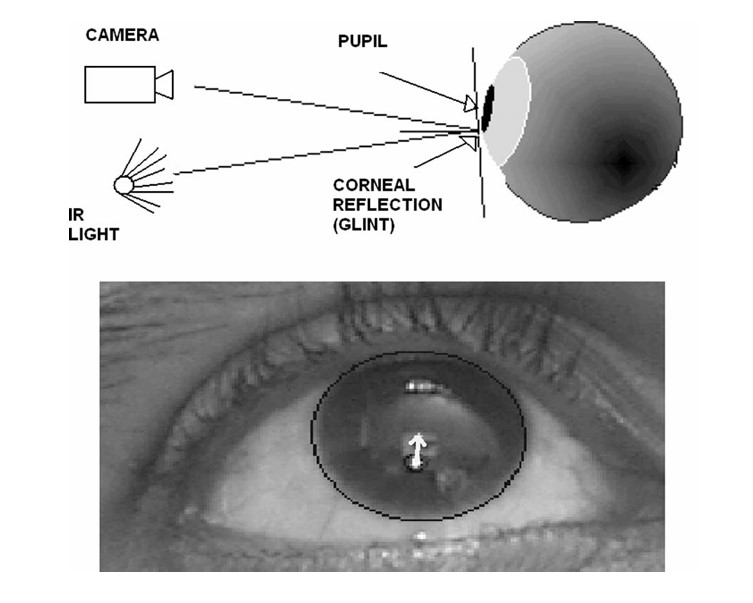
\includegraphics[width=0.8\columnwidth]{Chapter2/pccr.jpg}
    \caption{Sơ đồ biểu diễn kỹ thuật PCCR (ở trên) và vectơ ước tính từ tâm mống mắt đến điểm phản xạ \cite{sigut2010iris}}
    \label{fig:pccr}
\end{figure}

Trong những năm gần đây, theo dõi chuyển động mắt nhận được sự chú ý mạnh mẽ từ cộng đồng nghiên cứu. Những công bố từ các lĩnh vực khác nhau như tâm lý, giáo dục đặc biệt, v.v. đều sử dụng theo dõi chuyển động mắt như một công cụ đáng tin cậy cho việc khám phá những câu hỏi có liên quan đến việc phân bố sự chú ý trực quan. Chuyển động mắt được theo dõi và ghi nhận thông qua máy theo dõi chuyển động mắt (eye tracker). Trong số các kỹ thuật được áp dụng để theo dõi và ghi nhận chuyển động mắt, phương pháp Trung tâm đồng tử phản xạ giác mạc (Pupil Center Corneal Reflection - PCCR) là kỹ thuật phổ biến nhất và được tích hợp rộng rãi trong các thiết bị theo dõi chuyển động mắt hiện đại \cite{punde2017study, sigut2010iris}. Hình \ref{fig:pccr} minh họa một mô hình thiết lập điển hình của phương pháp PCCR. Góc của trục thị giác được xác định dựa trên vị trí tương đối giữa tâm đồng tử và điểm phản xạ trên giác mạc, với giả định rằng điểm phản xạ trên giác mạc sẽ không thay đổi khi vị trí của camera và nguồn sáng là cố định. Do đó, khi mắt xoay làm thay đổi vị trí của tâm đồng tử, góc tạo bởi tâm đồng tử và điểm phản xạ giác mạc cũng thay đổi tương ứng, từ đó cho phép tính toán chuyển động của mắt. Bên cạnh đó, nhiều thiết bị theo dõi chuyển động mắt hiện đại sử dụng nguồn sáng hồng ngoại nhằm tăng độ chính xác trong việc phát hiện tâm đồng tử, đồng thời giảm thiểu ảnh hưởng từ các yếu tố gây nhiễu như kính điều chỉnh tật khúc xạ hoặc ánh sáng môi trường.

% -------------------------------------------------------------------
% Area of Interest
% -------------------------------------------------------------------
\subsection{Nhận diện khu vực quan tâm}
\label{subsec:aoi}
Trong các nghiên cứu ứng dụng công nghệ theo dõi chuyển động mắt, thuật ngữ "khu vực quan tâm" (Areas of Interest – AOI) là một khái niệm phổ biến và đóng vai trò quan trọng. Khu vực quan tâm đề cập đến những vùng xác định, có thể có hình dạng bất kỳ, bao quanh các đối tượng cụ thể trong kích thích thị giác mà người quan sát tập trung ánh nhìn vào \cite{lagmay2022enhanced}. Việc phân tích chuyển động mắt trên toàn bộ kích thích thường tốn nhiều công sức và khó làm nổi bật được các đặc trưng liên quan đến từng yếu tố trong kích thích thị giác. Do đó, việc tập trung phân tích theo khu vực quan tâm giúp cung cấp các thước đo cục bộ, hỗ trợ hiệu quả hơn cho các nghiên cứu về sự chú ý và mức độ tập trung \cite{hessels2016area}. Các chỉ số định lượng từ khu vực quan tâm, chẳng hạn như thời gian nhìn chăm chú (dwell time), góp phần làm cho dữ liệu chuyển động mắt dễ phân tích và diễn giải hơn, đồng thời được ứng dụng rộng rãi trong nhiều lĩnh vực nghiên cứu như tương tác người–máy và tâm lý học \cite{hessels2016area}. Lý tưởng nhất là mỗi khu vực quan tâm nên có đường viền trùng khớp với hình dạng thực tế của đối tượng được quan sát, tuy nhiên, do một số đối tượng có hình dạng hoặc kích thước phức tạp và khó xác định chính xác, các khu vực quan tâm trong thực tế thường được biểu diễn bằng các hình học đơn giản như hình chữ nhật, hình elip, v.v. \cite{mahanama2022eye}.

Trong các nghiên cứu liên quan đến hội chứng rối loạn đọc, khu vực quan tâm thường được xác định tại các vùng chứa văn bản, chẳng hạn như toàn bộ đoạn văn (được xác định là vùng văn bản mở rộng khoảng 0.5 cm xung quanh) \cite{bonifacci2023eye}, các câu đơn lẻ trong văn bản \cite{bonifacci2023eye, raatikainen2021detection}, hoặc các từ riêng lẻ \cite{luniewska2022effect}. Bên cạnh đó, khu vực quan tâm cũng được áp dụng trong một số nghiên cứu về khả năng xử lý khuôn mặt ở trẻ mắc chứng rối loạn đọc, với dữ liệu đầu vào là hình ảnh hoặc video \cite{galazka2021facial, aasberg2022left}.


% -------------------------------------------------------------------
% Optical character recognition
% -------------------------------------------------------------------
\subsection{Nhận diện ký tự quang học}
\label{subsec:ocr}
Như đã trình bày trong mục \ref{subsec:aoi}, trong các bài toán ứng dụng công nghệ theo dõi chuyển động mắt nhằm hỗ trợ người mắc chứng rối loạn đọc, các khu vực quan tâm thường được xác định tại những vùng chứa văn bản. Trong những năm gần đây, nhờ sự phát triển mạnh mẽ của các kỹ thuật thị giác máy tính, việc xác định các khu vực quan tâm một cách tự động đã trở nên ngày càng dễ dàng. Đối với các khu vực liên quan đến văn bản, các thuật toán nhận dạng ký tự quang học (Optical Character Recognition – OCR) thường được sử dụng. Nhận dạng ký tự quang học là quá trình chuyển đổi hình ảnh điện tử của văn bản viết tay, đánh máy hoặc in ấn thành dạng văn bản mà máy tính có thể xử lý và hiểu được \cite{singh2012survey}. Phương pháp nhận dạng ký tự quang học cho phép tự động trích xuất thông tin từ văn bản và nhập vào cơ sở dữ liệu điện tử, thay thế cho việc nhập liệu thủ công. Công nghệ này đã được ứng dụng rộng rãi trong nhiều lĩnh vực như pháp luật (số hóa tài liệu pháp lý), ngân hàng (xử lý séc tự động), và chăm sóc sức khỏe (trích xuất thông tin từ biểu mẫu bệnh nhân), giúp tăng hiệu quả xử lý dữ liệu và giảm thiểu thời gian cũng như công sức.

\begin{figure}[h]
    \centering
    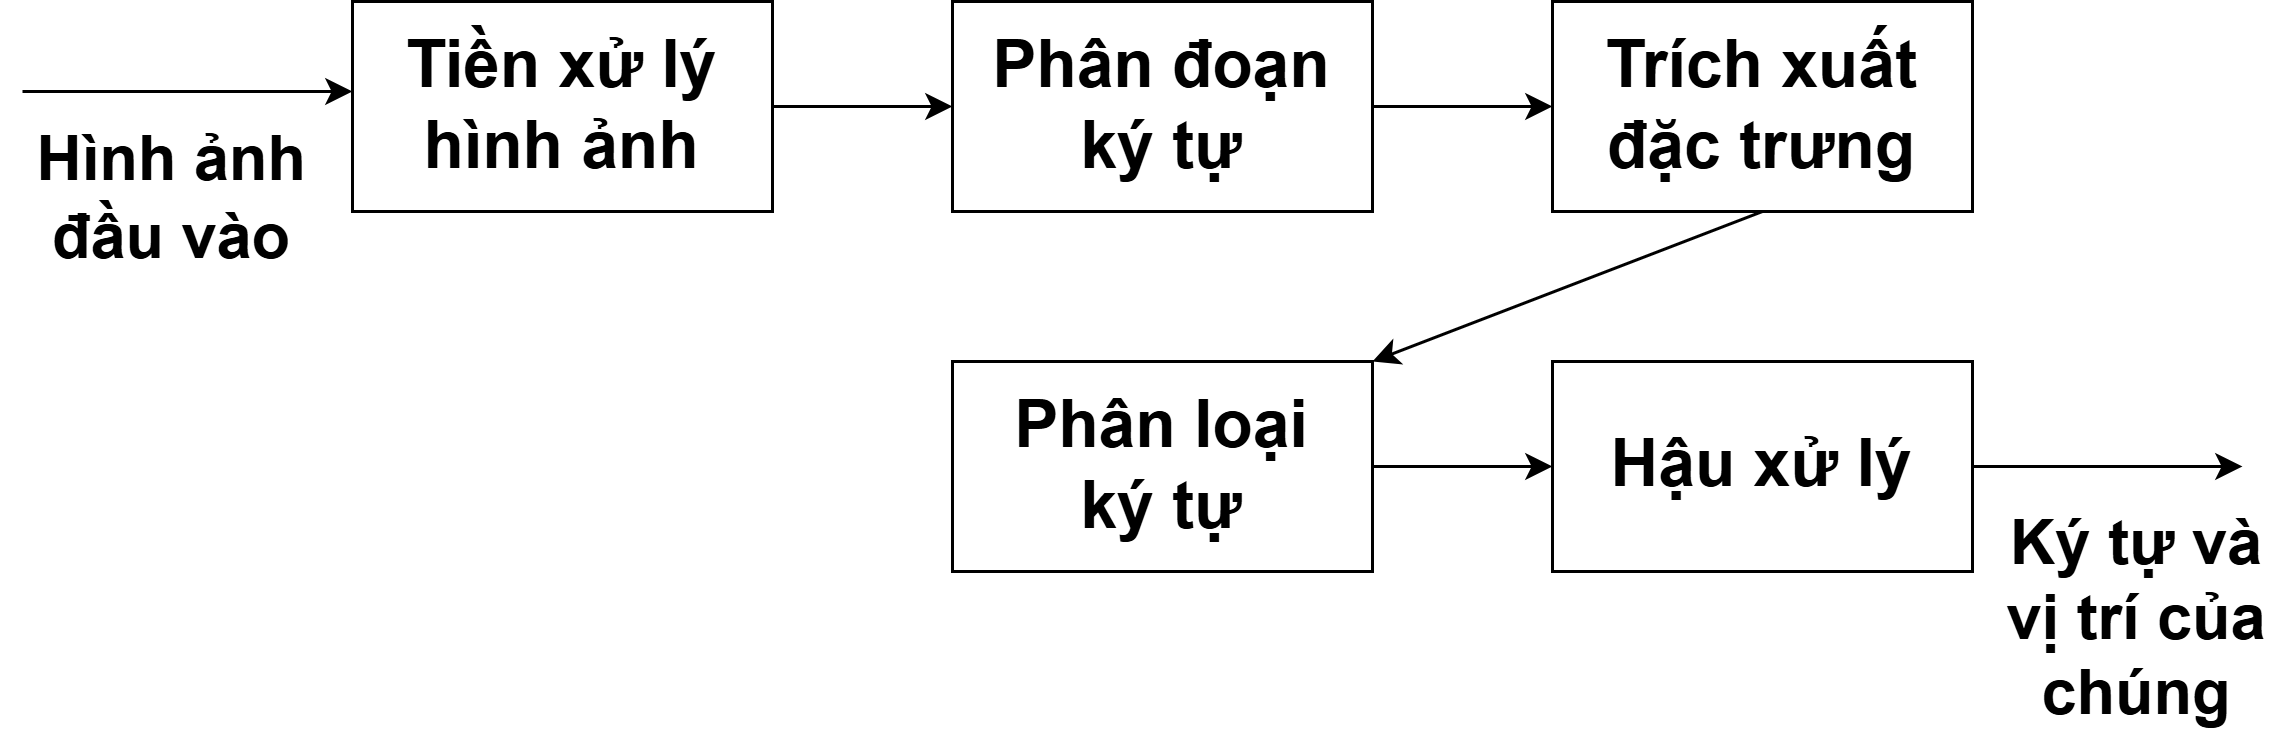
\includegraphics[width=0.8\columnwidth]{Chapter2/ocr.png}
    \caption{Tổng quan quy trình của thuật toán nhận dạng ký tự quang học}
    \label{fig:ocr}
\end{figure}

Có nhiều phương pháp nhận dạng ký tự quang học với các cách tiếp cận khác nhau, tuy nhiên, phần lớn các thuật toán đều tuân theo một quy trình gồm các bước cơ bản sau: thu thập hình ảnh, tiền xử lý, phân đoạn ký tự, trích xuất đặc trưng, phân loại ký tự và hậu xử lý \cite{islam2017survey}. Quá trình này được minh họa trong Hình \ref{fig:ocr}. Đầu tiên, hình ảnh văn bản được thu thập từ các nguồn khác nhau như văn bản in hoặc viết tay. Ở bước tiền xử lý, các kỹ thuật như chỉnh thẳng, phân tích bố cục hoặc phân ngưỡng được sử dụng để xử lý và làm sạch hình ảnh nguồn ở mức tổng thể, giúp văn bản dễ nhận diện hơn và giảm thiểu hoặc loại bỏ nhiễu. Sau đó, các ký tự được phân đoạn để tách riêng và chuẩn bị cho bước nhận dạng bằng các kỹ thuật như phân tích thành phần kết nối và hình chiếu. Tại bước trích xuất đặc trưng, hệ thống xác định các đặc điểm có khả năng phân biệt giữa các ký tự. Các đặc trưng này sau đó được đưa vào bộ phân loại để nhận dạng ký tự tương ứng dựa trên các kỹ thuật như phân loại cấu trúc, phân loại mẫu, v.v. Cuối cùng, bước hậu xử lý được áp dụng nhằm tinh chỉnh và nâng cao độ chính xác của kết quả nhận dạng. 




\subsection{Các đặc trưng của chuyển động mắt}
\label{subsec:emvm}

Trong các bài toán liên quan đến chuyển động mắt, việc tìm hiểu và lựa chọn các đặc trưng chuyển động mắt phù hợp là yếu tố hết sức quan trọng. Vì vậy, trong nội dung tiếp theo, khóa luận sẽ trình bày các hiểu biết liên quan đến những đặc trưng chuyển động mắt thường được sử dụng trong các nghiên cứu ứng dụng công nghệ theo dõi chuyển động mắt nhằm hỗ trợ người mắc chứng rối loạn đọc, bao gồm điểm nhìn, điểm dừng, đường trượt và hồi quy.

\begin{figure}[h]
    \centering
    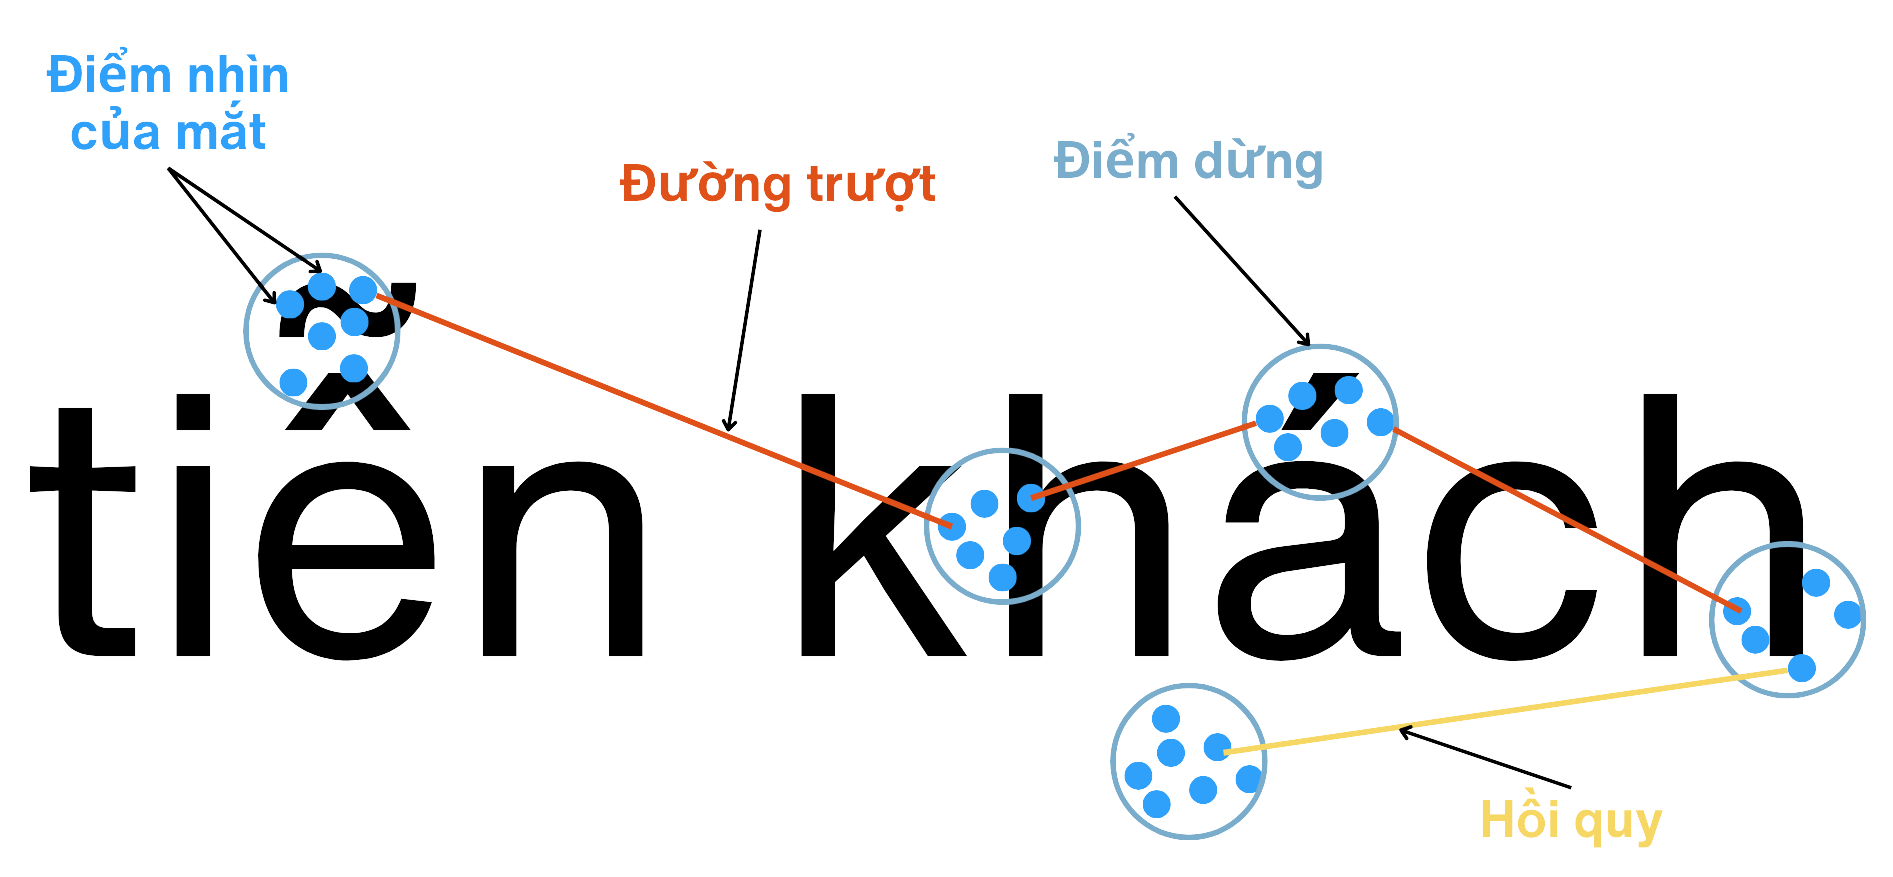
\includegraphics[width=0.9\columnwidth]{Chapter2/features.png}
    \caption{Các đặc trưng của chuyển động mắt: điểm nhìn của mắt, điểm dừng, đường trượt và hồi quy}
    \label{fig:features}
\end{figure}

\subsubsection{Điểm nhìn của mắt (Eye-gaze)}
Trong các nghiên cứu ứng dụng công nghệ theo dõi chuyển động mắt, phần lớn các thiết bị ghi nhận chuyển động mắt đều thu thập dữ liệu dưới dạng các điểm nhìn, biểu thị bởi các tọa độ \(x - y\) trên màn hình kèm theo thông tin thời gian tương ứng với từng điểm nhìn. Số lượng điểm nhìn thu được tỷ lệ thuận với khoảng thời gian người tham gia quan sát màn hình. Tuy nhiên, trong nhiều trường hợp, dữ liệu điểm nhìn có thể gây ra những khó khăn nhất định cho các nhà nghiên cứu do mật độ điểm quá lớn, dẫn đến khó khăn trong việc phân tích và phát hiện các đặc điểm đáng chú ý. Do đó, tùy vào mục tiêu cụ thể và phương pháp tiếp cận của từng nghiên cứu, dữ liệu điểm nhìn có thể được sử dụng trực tiếp hoặc được xử lý để trích xuất các đặc trưng trung gian giúp việc quan sát và phân tích trở nên hiệu quả hơn. Một số đặc trưng phổ biến thường được sử dụng bao gồm: điểm dừng, đường trượt và hồi quy, được minh họa trong Hình \ref{fig:features}.


\subsubsection{Điểm dừng (Fixation)}
\label{subsubsec:fix}
Điểm dừng là đặc trưng mà mắt của con người nhìn cố định vào một mục tiêu thị giác cụ thể, đồng thời duy trì sự ổn định trong nhận thức và tiếp nhận thông tin thị giác của mắt \cite{rayner200935th}. Quá trình tính toán điểm dừng giúp đơn giản hóa đáng kể dữ liệu chuyển động mắt bằng cách hợp nhất các điểm riêng lẻ thành một điểm dữ liệu hợp nhất \cite{salvucci2000identifying}. Vì vậy, việc sử dụng điểm dừng góp phần đơn giản hóa tập dữ liệu, đồng thời vẫn bảo toàn các đặc trưng cốt lõi có giá trị trong phân tích và nghiên cứu.

Nhiều đặc trưng thống kê của điểm dừng được sử dụng trong phân tích chuyển động mắt, tùy thuộc vào từng vấn đề cụ thể, bao gồm số lượng điểm dừng, thời lượng điểm dừng, vị trí của điểm dừng tại mỗi từ, v.v, mỗi chỉ số phản ánh các khía cạnh khác nhau của hành vi thị giác \cite{poole2006eye}. Chẳng hạn, số lượng điểm dừng và thời lượng của mỗi điểm dừng phản ánh quá trình nhận thức và xử lý ngôn ngữ ở thời gian thực. Số lượng điểm dừng ít và thời lượng điểm dừng ngắn cho thấy quá trình xử lý song song diễn ra tốt, vì trong khi đọc, việc xử lý văn bản và định hướng chuyển động mắt diễn ra đồng thời \cite{poole2006eye}. Trong nhiều thí nghiệm, trẻ rối loạn đọc thường cho thấy các đặc trưng thống kê điểm dừng khác biệt, chẳng hạn như thời lượng điểm dừng dài hơn và số lượng điểm dừng nhiều hơn so với trẻ phát triển bình thường. Những quan sát này cho thấy rằng nhóm trẻ này cần nhiều thời gian hơn để phân tích, thu thập thông tin, nhận thức và xử lý từ vựng \cite{parshina2022global},  cũng như khả năng phối hợp chuyển động mắt kém hiệu quả hơn \cite{kirkby2008binocular}.


\subsubsection{Đường trượt (Saccade)}
\label{subsubsec:sac}
Đường trượt là đặc trưng về chuyển động nhanh của mắt di chuyển từ một điểm dừng này đến điểm dừng tiếp theo \cite{carter2020best}. Nhiều nghiên cứu đã chỉ ra rằng sự điều khiển tốt hệ thống đặc trưng chuyển động của mắt, trong đó có đường trượt và điểm dừng, là rất cần thiết cho việc đọc \cite{levy1979control}. Khi ta nhận biết hình ảnh, chúng ta sẽ thu thập thông tin tại mỗi điểm dừng và chuyển vùng lấy thông tin thông qua đường trượt. Đường trượt được ghi lại có thể phản ánh khoảng cách và mối liên hệ theo trật tự thời gian của tiến trình xử lý thông tin trong quá trình định danh hình ảnh \cite{roitsch2019overview}. 

Trẻ rối loạn đọc thường có số đường trượt nhiều hơn và độ dài của mỗi đường trượt ngắn hơn khi so sánh với những trẻ phát triển bình thường. Nguyên nhân của việc thực hiện nhiều đường trượt là do sự hạn chế về mặt nhạy bén trong quá trình xử lý thông tin thị giác \cite{seassau2014binocular}. Ngoài ra, độ dài của đường trượt lớn còn cho thấy khả năng đọc trôi chảy và tự tin, trong khi đó đường trượt nhỏ biểu thị khả năng đọc khó khăn \cite{smyrnakis2021silent}.


\subsubsection{Hồi quy (Regression)}
\label{subsubsec:reg}
Hồi quy, hay còn gọi là chuyển động giật lùi của mắt (regressive saccade), là một đặc trưng thị giác đại diện cho chuyển động của mắt theo hướng ngược lại với tiến trình đọc hoặc quan sát. Đối với người đọc bình thường, hồi quy thường xuất hiện tại điểm dừng cuối cùng của một dòng văn bản và hướng về các điểm dừng nằm ở phía bên trái của các vị trí đó \cite{booth2013function}.

Sự xuất hiện của các chuyển động hồi quy có thể bắt nguồn từ nhiều nguyên nhân khác nhau. Trước hết, trong quá trình đọc, mắt có thể bỏ qua những từ mang thông tin quan trọng hoặc rời khỏi điểm dừng trước khi quá trình xử lý thông tin thị giác hoàn tất, dẫn đến sự không chắc chắn trong việc tiếp nhận nội dung \cite{inhoff2019regressions}. Hiện tượng này thường được quan sát thấy rõ hơn khi người đọc xử lý các văn bản có cấu trúc phức tạp, chứa lỗi ngữ pháp hoặc mang nội dung mơ hồ, những yếu tố làm gia tăng mức độ không chắc chắn về mặt thông tin \cite{inhoff2009word}. Bên cạnh đó, hồi quy còn liên hệ chặt chẽ với năng lực trí nhớ công việc (working memory), khi nó đóng vai trò như một cơ chế hỗ trợ người đọc hồi tưởng lại những thông tin đã đọc trước đó, đặc biệt trong trường hợp các văn bản dài và đòi hỏi khả năng lưu giữ và tích hợp thông tin cao \cite{spivey2013thinking}. Trong các nghiên cứu về rối loạn đọc, người mắc chứng này thường có tần suất hồi quy cao hơn đáng kể so với người đọc bình thường, phản ánh quá trình xử lý, tiếp nhận và hiểu văn bản kém hiệu quả hơn, cũng như những hạn chế về trí nhớ công việc.


\subsection{Các phương pháp trực quan hoá}
\label{subsec:visual}
Các đặc trưng của chuyển động mắt được trình bày tại Mục \ref{subsec:emvm} thường là các đặc trưng mang tính thống kê. Để trực quan hóa những đặc trưng này, các phương pháp như bản đồ nhiệt và đường quét thường được sử dụng trong các bài toán ứng dụng công nghệ theo dõi chuyển động mắt để hỗ trợ người mắc chứng rối loạn đọc. Trong nội dung tiếp theo, khóa luận sẽ trình bày tổng quan về hai phương pháp trực quan hóa phổ biến này. 
\subsubsection{Bản đồ nhiệt (Heatmap)}
\label{subsubsec:heatmap}

Một trong những phương pháp trực quan hóa dữ liệu được ứng dụng rộng rãi trong các nghiên cứu sử dụng công nghệ theo dõi chuyển động mắt là bản đồ nhiệt. Bản đồ nhiệt phản ánh phân bố không gian của chuyển động mắt trên các kích thích thị giác, mà không bao hàm yếu tố thời gian, từ đó cung cấp cái nhìn tổng quan về hành vi quan sát của người tham gia. Trong bối cảnh nghiên cứu chứng rối loạn đọc, bản đồ nhiệt đặc biệt hữu ích trong việc xác định những vùng mà trẻ tập trung ánh nhìn nhiều hơn (hoặc ít hơn) trên ngữ liệu kích thích, qua đó cho phép đánh giá mức độ chú ý hoặc những khu vực đòi hỏi nhiều nỗ lực nhận diện và xử lý ngôn ngữ hơn từ phía trẻ \cite{mahanama2022eye}. Trong thực tiễn, bản đồ nhiệt thường được biểu diễn dưới dạng Mô hình Hỗn hợp Gaussian (Gaussian Mixture Model - GMM), nhằm mô tả xác suất hoặc tần suất xuất hiện của các điểm dừng mắt. Việc sử dụng GMM trong trực quan hóa dữ liệu sẽ được trình bày chi tiết tại Mục \ref{subsec:visualizee}. Kết quả của quá trình này được hiển thị thông qua một mặt nạ mã hóa màu được chồng lên hình ảnh kích thích thị giác mà người tham gia quan sát. Các vùng có màu “nóng” (chẳng hạn như đỏ, cam hoặc vàng) biểu thị sự tập trung cao hơn, trong khi các màu “lạnh” (như xanh lá cây) phản ánh mức độ chú ý thấp hơn \cite{mahanama2022eye}.

Thông thường, bản đồ nhiệt chủ yếu được ứng dụng trong các nghiên cứu liên quan đến hành vi quan sát trên các giao diện người dùng, chẳng hạn như trang web hoặc công cụ tìm kiếm thông tin, trong khi việc sử dụng bản đồ nhiệt trong các nghiên cứu về hỗ trợ trẻ mắc chứng rối loạn đọc, đặc biệt với ngôn ngữ tiếng Anh, vẫn còn hạn chế. Tuy nhiên, do sự khác biệt đáng kể giữa tiếng Việt và tiếng Anh đã được trình bày trong phần Đặt vấn đề, nghiên cứu này khai thác bản đồ nhiệt như một công cụ trực quan để phân tích hành vi quan sát của trẻ, nhằm xác định các vần trong một từ mà trẻ tập trung nhìn vào nhiều hơn hoặc mất nhiều thời gian hơn để xử lý.

\begin{figure}[h]
    \centering
    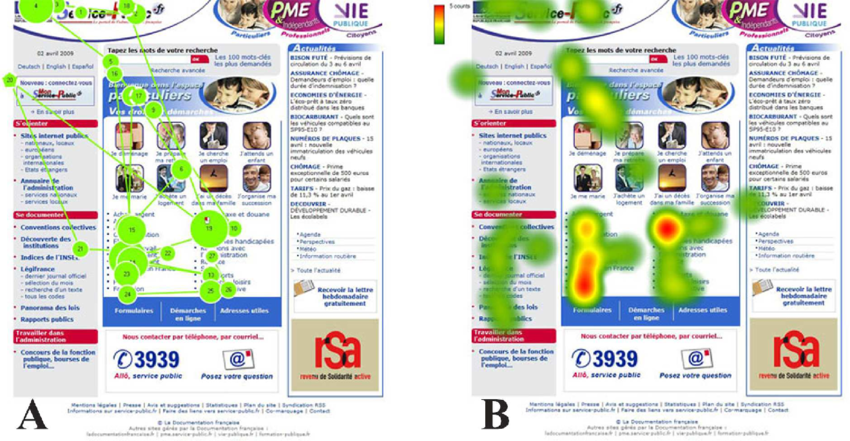
\includegraphics[width=\columnwidth]{Chapter2/heatmap-scanpath.png}
    \caption{Hình ảnh đường quét (trái) và bản đồ nhiệt (phải) thể hiện dữ liệu chuyển động mắt của người dùng trên một trang web \cite{drusch2014analysing}}
    \label{fig:heatmap-scanpath}
\end{figure}

\subsubsection{Đường quét (Scan path)}
\label{subsubsec:scanpath}
Đường quét thể hiện mô hình chuyển động của mắt trong một nhiệm vụ thị giác, phản ánh cả hai chiều không gian và thời gian thông qua chuỗi các điểm dừng và đường trượt. Khác với bản đồ nhiệt chỉ cung cấp tổng quan về mật độ quan sát, đường quét cho phép phân tích chi tiết hơn về hành vi nhìn, bao gồm các vị trí mà người tham gia tập trung sự chú ý, thứ tự quan sát, mức độ chú ý tại từng khu vực, cũng như chiến lược di chuyển ánh nhìn trên kích thích thị giác \cite{mahanama2022eye}. Thông thường, đường quét được biểu diễn dưới dạng chuỗi các nút (đại diện cho vị trí điểm dừng) và các cạnh kết nối (đại diện cho đường trượt giữa các điểm dừng liên tiếp), được phủ trực tiếp lên ngữ liệu thị giác, với đường kính của mỗi nút thường tỉ lệ thuận với thời gian cố định tại vị trí đó \cite{goldberg2010scanpath}. Phân tích đường quét đã được ứng dụng rộng rãi trong nhiều lĩnh vực như sinh trắc học, khoa học thần kinh, và đặc biệt là trong các nghiên cứu về rối loạn đọc. Al-Wabil và cộng sự \cite{al2008examining} chỉ ra rằng những người mắc chứng rối loạn đọc có xu hướng có các đường quét không ổn định hơn, cũng như ít mang tính chiến lược hơn khi tương tác với các cấu trúc điều hướng trên giao diện web. Ngoài ra, nghiên cứu của Parshina và cộng sự \cite{appadurai2022image} cũng cho thấy mặc dù có những đặc điểm chung trong các đường quét giữa các cá nhân, vẫn tồn tại sự khác biệt đáng kể phản ánh phong cách đọc riêng biệt của từng người. Từ đó, đường quét được xem là một công cụ giàu tiềm năng để phân tích sự khác biệt giữa các cá nhân hoặc nhóm đối tượng thông qua dữ liệu chuyển động mắt. Ví dụ về đường quét và bản đồ nhiệt được thể hiện ở Hình \ref{fig:heatmap-scanpath}.

% -------------------------------------------------------------------
% Chapter summary
% -------------------------------------------------------------------
\section{Kết chương}
Chương này đã trình bày các hiểu biết về rối loạn đọc, cũng như những kiến thức nền tảng về công nghệ được sử dụng để phát triển giải pháp trong khóa luận, bao gồm công nghệ theo dõi chuyển động mắt, khu vực quan tâm, thuật toán nhận diện ký tự quang học, các đặc trưng của chuyển động mắt, cũng như các phương pháp trực quan hoá. 

\chapter{Phương pháp nghiên cứu và giải pháp đề xuất}
\label{chap:method-solution}

Chương này trình bày phương pháp nghiên cứu và giải pháp đề xuất cho bài toán tối ưu bộ luật WAF ModSecurity trong phát hiện Cross-Site Scripting và SQL Injection. Nếu Chương 2 xây dựng nền tảng về WAF, ModSecurity, OWASP CRS, XSS, SQLi và các hướng phát hiện liên quan, thì chương này mô tả cách khóa luận tiếp cận bài toán và thiết kế bộ generalized rules v2. Nội dung bắt đầu từ quy trình nghiên cứu tổng thể, sau đó trình bày nguyên tắc phương pháp luận, kiến trúc giải pháp, thiết kế XSS/SQLi rules, decode pipeline, tích hợp anomaly scoring và phương pháp tuning.

Chương này không đi sâu vào môi trường chạy thí nghiệm, dataset hay công cụ benchmark. Các nội dung đó được trình bày ở Chương 4 sau khi giải pháp đã được mô tả đầy đủ. Cách sắp xếp này giúp mạch luận văn đi từ vấn đề và phương pháp đề xuất tới thiết kế đánh giá, phù hợp hơn với cấu trúc của một bài báo khoa học hoặc đồ án kỹ thuật.

\section{Tổng quan quy trình nghiên cứu}
\label{sec:research-workflow}

Quy trình nghiên cứu của khóa luận được xây dựng theo hướng lặp: phân tích hệ thống hiện có, thiết kế cải tiến, đánh giá định lượng, phân tích lỗi và tiếp tục tuning. Cách tiếp cận này phù hợp với bài toán tối ưu WAF vì chất lượng của rule không thể được đánh giá chỉ bằng cách đọc regex. Một rule có thể hợp lý ở mức cú pháp nhưng vẫn bỏ sót payload bị mã hóa, hoặc chặn nhầm nhiều request hợp lệ khi chạy trên dữ liệu thực tế. Do đó, mỗi thay đổi trong rule cần được kiểm chứng bằng benchmark và audit log~\cite{benchmark-methodology,waf-tuning-methodology}.

Hình~\ref{fig:research-pipeline-flow} mô tả luồng nghiên cứu tổng quát. Quy trình bắt đầu từ việc khảo sát OWASP CRS và các rule gốc theo hướng enumeration-based. Từ đó, các false negative và false positive được phân tích để xác định hạn chế của cách phát hiện dựa trên danh sách cố định. Tiếp theo, khóa luận thiết kế bộ generalized rules v2 cho XSS và SQLi, tích hợp rule với anomaly scoring của CRS, xây dựng phương pháp tuning dựa trên dữ liệu và cuối cùng thiết kế thực nghiệm để đánh giá giải pháp.

\begin{figure}[p]
    \centering
    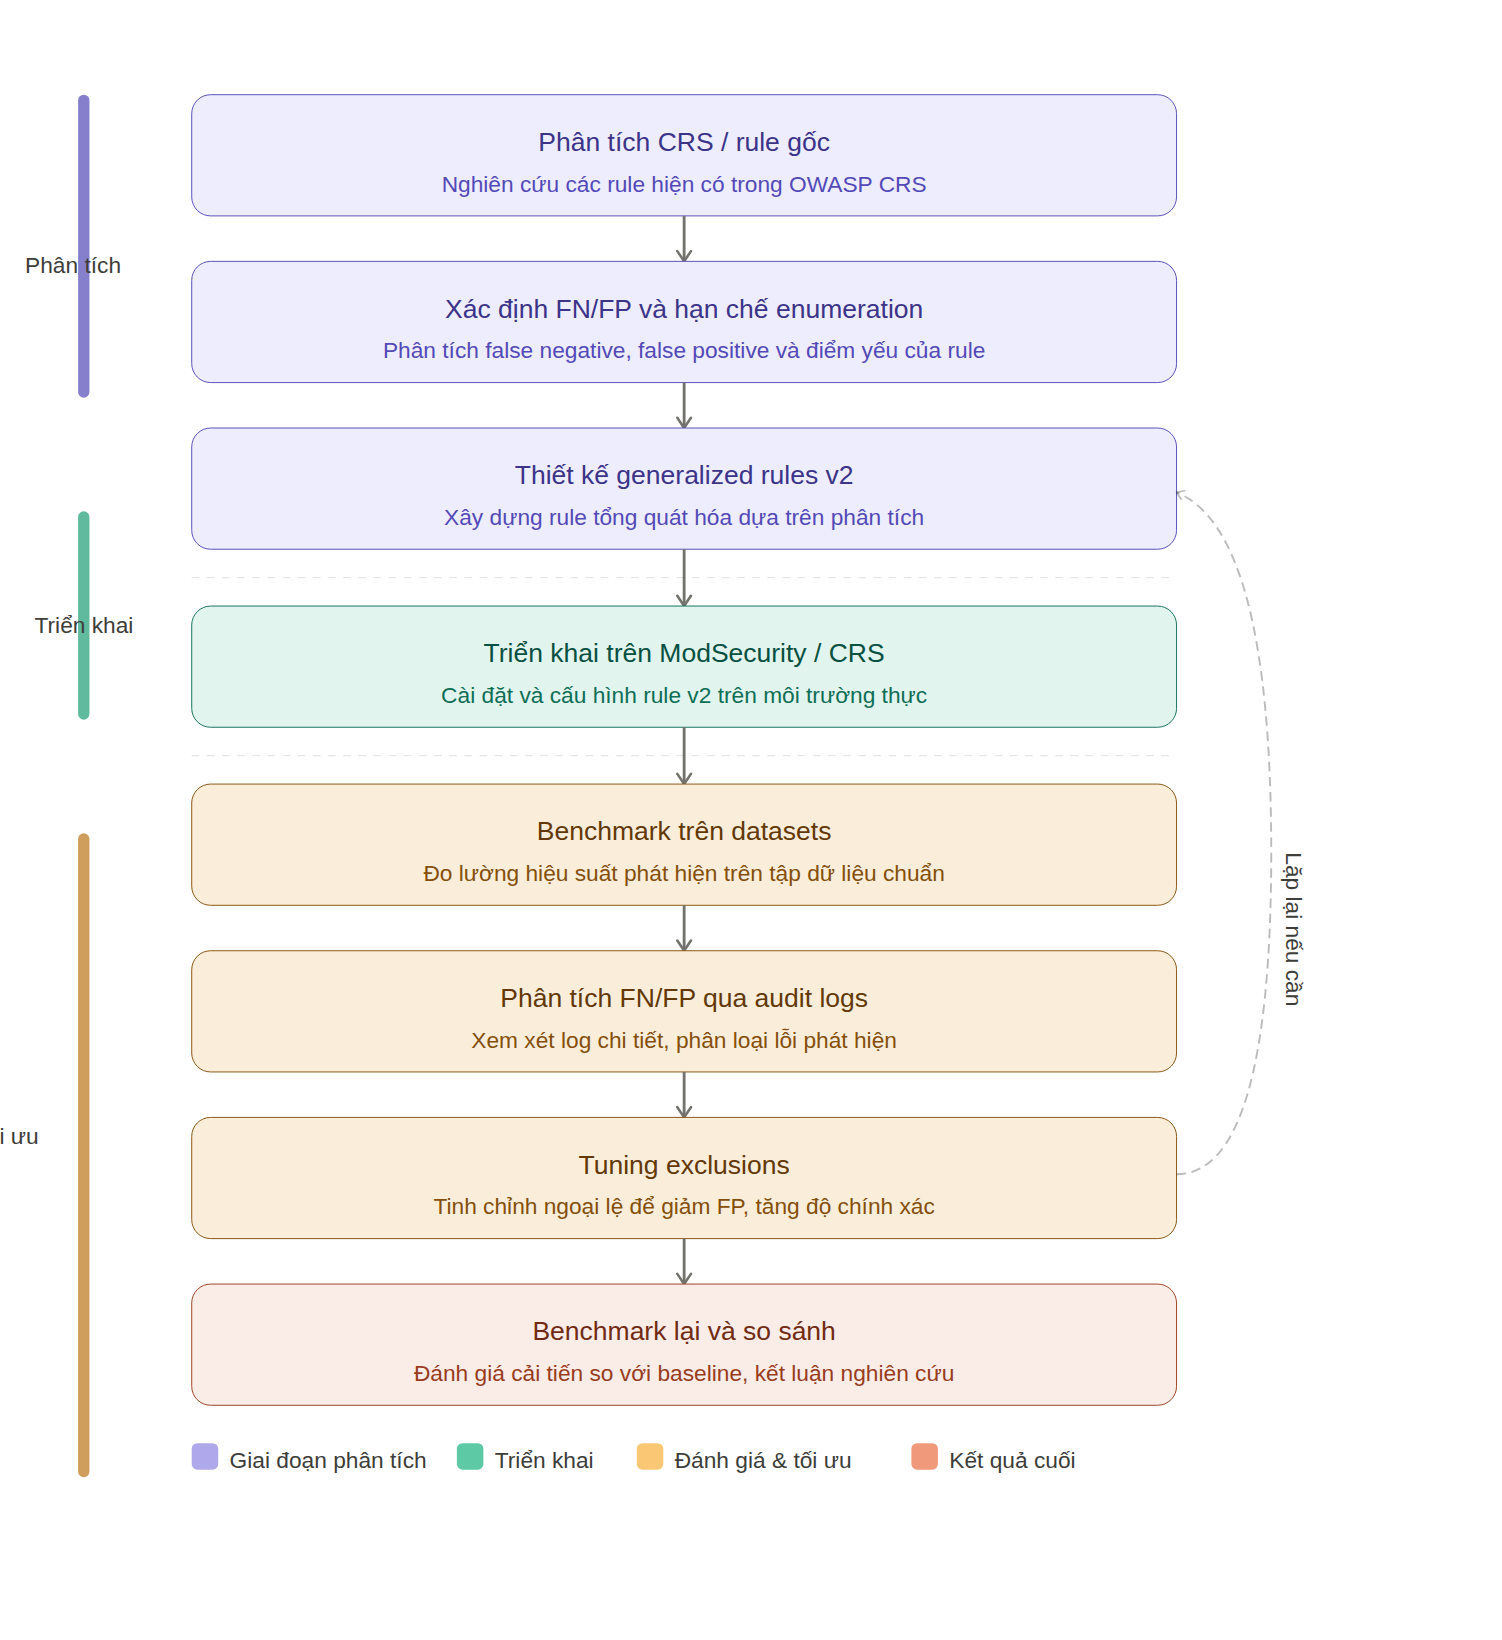
\includegraphics[width=0.92\textwidth,height=0.80\textheight,keepaspectratio]{Chapter3/research_pipeline_flow.png}
    \caption{Quy trình nghiên cứu tổng quát của khóa luận}
    \label{fig:research-pipeline-flow}
\end{figure}

Có thể chia quy trình trên thành ba giai đoạn chính. Giai đoạn thứ nhất là phân tích, bao gồm tìm hiểu CRS, rule gốc và các nhóm payload gây lỗi. Giai đoạn thứ hai là đề xuất giải pháp, bao gồm thiết kế rule v2, decode pipeline, anomaly scoring integration và tuning methodology. Giai đoạn thứ ba là đánh giá, bao gồm thiết kế môi trường thực nghiệm, chạy benchmark, phân tích FN/FP và so sánh với baseline. Chương này tập trung vào hai giai đoạn đầu; Chương 4 trình bày chi tiết giai đoạn đánh giá.

\section{Nguyên tắc phương pháp luận}
\label{sec:methodological-principles}

Phương pháp nghiên cứu của khóa luận dựa trên bốn nguyên tắc chính.

Thứ nhất, việc tối ưu WAF phải dựa trên dữ liệu thay vì chỉ dựa trên trực giác viết rule. Các false negatives cho biết rule còn bỏ sót kỹ thuật nào; các false positives cho biết rule nào quá rộng hoặc không phù hợp với traffic mục tiêu. Vì vậy, benchmark và audit log không chỉ được dùng để báo cáo kết quả cuối cùng, mà còn là công cụ để cải thiện rule theo vòng lặp.

Thứ hai, khóa luận ưu tiên generalized/context-aware detection thay vì enumeration-based detection. Với XSS, rule cần phát hiện ngữ cảnh thực thi như thẻ có khả năng chạy mã, event handler có giá trị nguy hiểm, protocol URI hoặc DOM sink. Với SQLi, rule cần phát hiện semantic patterns như \path|UNION SELECT|, stacked query, boolean bypass, time-based function hoặc schema enumeration. Cách tiếp cận này nhằm giảm phụ thuộc vào danh sách payload cố định.

Thứ ba, mục tiêu đánh giá không chỉ là tối đa hóa recall. Trong WAF, false positive rate có ý nghĩa vận hành rất lớn: một hệ thống chặn được nhiều payload tấn công nhưng đồng thời chặn nhầm nhiều request hợp lệ sẽ khó triển khai thực tế. Do đó, mọi cải tiến rule cần được đọc đồng thời qua recall, FPR, precision và các ví dụ FP/FN cụ thể.

Thứ tư, tuning CRS phải có kiểm soát. Việc dùng \path|SecRuleRemoveById| không được hiểu là tắt rule để làm đẹp chỉ số, mà là thay thế hoặc loại bỏ có chọn lọc các rule gây FP cao, trùng lặp với custom rules hoặc nằm ngoài phạm vi đánh giá. Mỗi quyết định tuning cần đi kèm bằng chứng từ benchmark, audit log và phân tích rủi ro.

\section{Kiến trúc tổng quan giải pháp}
\label{sec:solution-architecture}

Giải pháp được xây dựng trên kiến trúc WAF sử dụng ModSecurity kết hợp OWASP Core Rule Set. ModSecurity đóng vai trò WAF engine xử lý HTTP transaction, còn CRS cung cấp rule set nền, cơ chế anomaly scoring và rule chặn tổng hợp. Custom rules v2 được bổ sung vào cùng pipeline xử lý của CRS, thay vì hoạt động như một bộ lọc độc lập. Khi một rule v2 khớp với request, rule không chỉ ghi nhận dấu hiệu XSS/SQLi riêng mà còn cộng điểm vào biến inbound anomaly score của CRS. Quyết định cuối cùng Block/Pass vẫn dựa trên cơ chế threshold của CRS~\cite{modsecurity-docs,owasp-crs-docs,modsecurity-crs-overview}.

Hình~\ref{fig:modsecurity-architecture-flow} mô tả luồng xử lý tổng quát của giải pháp. HTTP request đi qua các phase của ModSecurity, được chuẩn hóa bởi các transformation cần thiết, sau đó được kiểm tra bởi hai nhóm custom rules chính: XSS generalized rules trong dải \path|9942xxx| và SQLi generalized rules trong dải \path|9943xxx|. Các rule này cộng điểm vào anomaly score tương ứng; sau đó CRS scoring engine, đặc biệt nhóm rule \path|949xxx|, đánh giá tổng điểm và quyết định request có bị chặn hay không.

\begin{figure}[p]
    \centering
    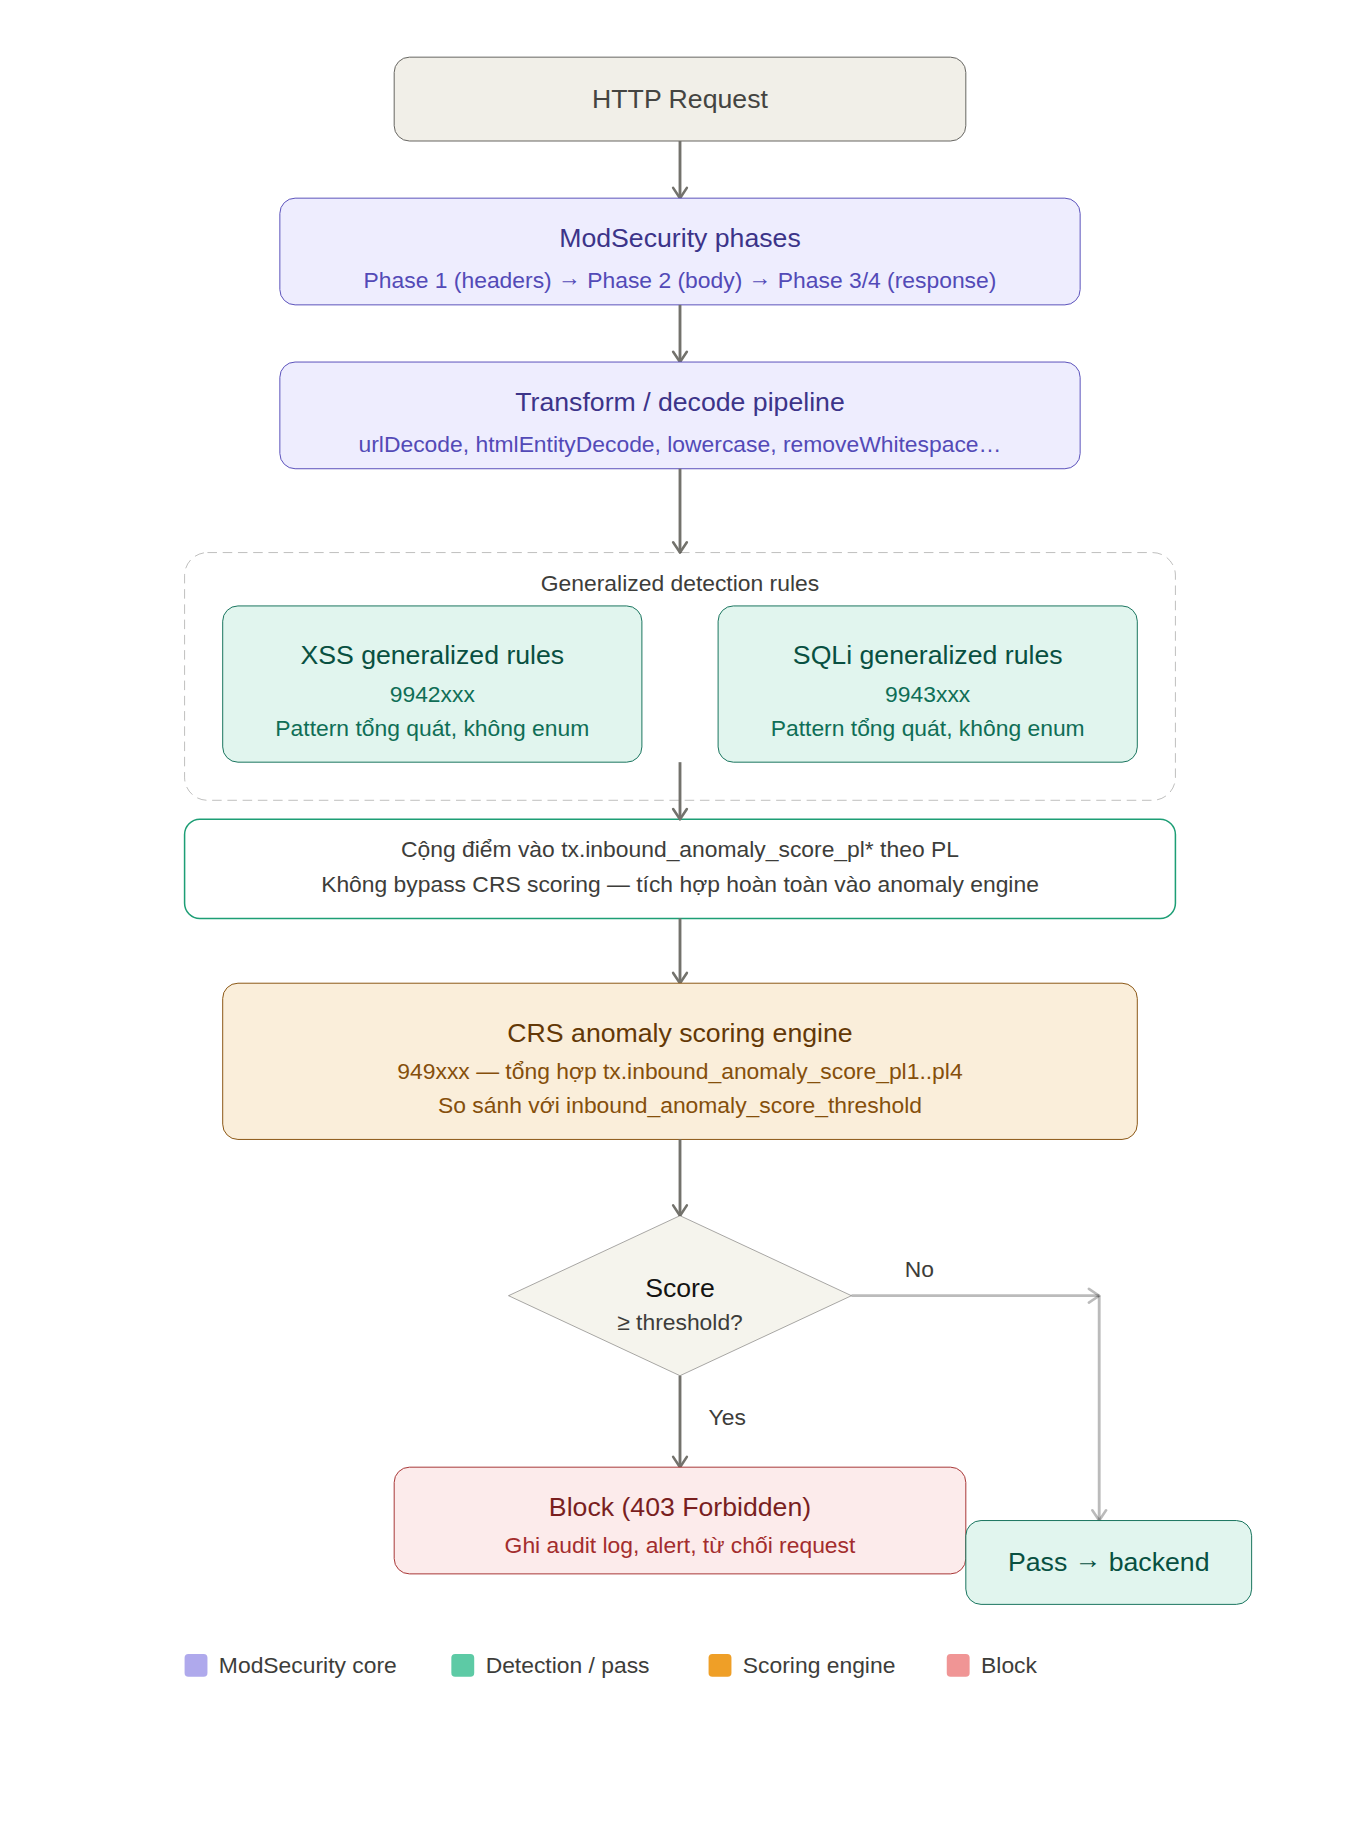
\includegraphics[width=0.92\textwidth,height=0.80\textheight,keepaspectratio]{Chapter4/modsecurity_architecture_flow.png}
    \caption{Kiến trúc xử lý request của giải pháp ModSecurity/CRS với generalized rules}
    \label{fig:modsecurity-architecture-flow}
\end{figure}

Bảng~\ref{tab:solution-logical-components} tóm tắt các thành phần logic trong giải pháp. Các chi tiết triển khai cụ thể như Docker image, backend thử nghiệm, tham số môi trường và audit log path được trình bày ở Chương 4 trong phần thiết kế thực nghiệm.

{\small
\renewcommand{\arraystretch}{1.2}
\begin{longtable}{|L{0.24\textwidth}|L{0.32\textwidth}|L{0.34\textwidth}|}
\caption{Các thành phần logic trong kiến trúc giải pháp}\label{tab:solution-logical-components}\\
\hline
\textbf{Thành phần} & \textbf{Vai trò} & \textbf{Ghi chú thiết kế} \\
\hline
\endfirsthead

\hline
\textbf{Thành phần} & \textbf{Vai trò} & \textbf{Ghi chú thiết kế} \\
\hline
\endhead

OWASP CRS nền & Cung cấp rule set tổng quát, anomaly scoring và rule đánh giá tổng điểm. & Không bị thay thế hoàn toàn; giải pháp chỉ chuyên biệt hóa phát hiện XSS/SQLi. \\
\hline
XSS generalized rules v2 & Phát hiện XSS theo hướng context-aware. & Dải ID \path|9942xxx|, tập trung vào execution context và payload encoded/obfuscated. \\
\hline
SQLi generalized rules v2 & Phát hiện SQLi theo hướng semantic-based. & Dải ID \path|9943xxx|, tập trung vào cấu trúc injection và coverage đa DBMS. \\
\hline
Decode pipeline & Chuẩn hóa payload trước khi so khớp. & Dùng URL decode, HTML entity decode, JavaScript decode, remove nulls, compress whitespace và Base64 decode có điều kiện. \\
\hline
Anomaly scoring integration & Cộng điểm vào CRS để quyết định block/pass theo threshold. & Rule v2 dùng severity khác nhau thay vì chặn mọi dấu hiệu với cùng mức độ. \\
\hline
Tuning exclusions & Giảm FP từ các CRS rules quá tổng quát hoặc trùng logic. & Được sử dụng có kiểm soát, dựa trên audit log và phân tích rủi ro. \\
\hline
\end{longtable}
}

Điểm quan trọng của kiến trúc này là custom rules v2 không thay thế toàn bộ CRS. Chúng được thiết kế để bổ sung và chuyên biệt hóa khả năng phát hiện XSS/SQLi, đồng thời tận dụng cơ chế scoring sẵn có của CRS. Việc tuning exclusions chỉ được áp dụng có chọn lọc trong phạm vi nghiên cứu để giảm nhiễu và giảm false positives, không phải khuyến nghị cấu hình mặc định cho mọi hệ thống production.

\section{Nguyên tắc thiết kế bộ luật v2}
\label{sec:rule-design-principles}

Bộ luật v2 được thiết kế theo hướng generalized thay vì enumeration-based. Cách tiếp cận enumeration-based thường mở rộng danh sách payload, từ khóa hoặc hàm đã biết. Cách này dễ triển khai ban đầu nhưng khó bao phủ các biến thể mới và dễ gây false positives khi pattern quá rộng. Ngược lại, generalized rules cố gắng mô tả cấu trúc hoặc ngữ cảnh tấn công ở mức tổng quát hơn: XSS được nhìn dưới góc độ execution context, còn SQLi được nhìn dưới góc độ semantic pattern của câu lệnh SQL bị chèn.

Nguyên tắc đầu tiên là context-aware detection cho XSS. Một chuỗi như \path|script|, \path|alert| hoặc \path|onload| không luôn là tấn công. Nó có thể xuất hiện trong tài liệu kỹ thuật, nội dung bài viết hoặc dữ liệu hợp lệ. Vì vậy, rule XSS v2 không chỉ kiểm tra sự tồn tại của từ khóa mà còn kiểm tra vị trí và ngữ cảnh thực thi, ví dụ thẻ \path|<script>| có nội dung thực thi, event handler có giá trị nguy hiểm, protocol URI \path|javascript:|, hoặc DOM sink như \path|innerHTML| đi kèm HTML/script injection.

Nguyên tắc thứ hai là semantic-based detection cho SQLi. SQLi v2 không bắt các keyword rời như \path|select| hoặc \path|or| một cách độc lập, vì các từ này có thể xuất hiện trong dữ liệu hợp lệ. Thay vào đó, rule tập trung vào các cấu trúc có ý nghĩa injection, chẳng hạn \path|UNION SELECT|, stacked query bắt đầu bằng dấu chấm phẩy và theo sau là DML/DDL keyword, quote kết hợp toán tử logic và tautology, hàm time-based blind SQLi hoặc truy cập system catalog.

Nguyên tắc thứ ba là chuẩn hóa dữ liệu trước khi so khớp. Payload tấn công có thể được URL encode, HTML entity encode, JavaScript escape, chèn null byte hoặc chèn khoảng trắng bất thường. Vì vậy, nhiều rule v2 sử dụng các transformation như \path|t:urlDecodeUni|, \path|t:htmlEntityDecode|, \path|t:jsDecode|, \path|t:removeNulls| và \path|t:compressWhitespace| trước khi áp dụng regex. Với Base64, giải pháp dùng các rule chuyên biệt để decode rồi kiểm tra lại nội dung đã decode, thay vì coi mọi chuỗi Base64 là tấn công.

Nguyên tắc thứ tư là hiệu chỉnh severity theo độ tin cậy của dấu hiệu. Các pattern có độ tin cậy cao như \path|UNION SELECT|, event handler gọi hàm nguy hiểm hoặc protocol URI \path|javascript:| được gán mức \path|CRITICAL|. Các pattern encoded/obfuscated hoặc error-based có thể gán \path|ERROR|. Các pattern context-specific hoặc heuristic nâng cao có thể gán \path|WARNING| hoặc \path|NOTICE|. Cách phân tầng này giúp rule v2 hòa vào anomaly scoring thay vì chặn mọi dấu hiệu với cùng mức nghiêm trọng.

Nguyên tắc cuối cùng là giảm false positives bằng cách giới hạn phạm vi input target và tổ chức rule dễ bảo trì. XSS v2 cố ý không scan \path|REQUEST_HEADERS:User-Agent| vì header này thường chứa chuỗi phức tạp từ trình duyệt, bot hoặc công cụ tự động, dễ gây FP nếu kiểm tra quá rộng. Các rule được chia theo dải ID và lớp kỹ thuật, giúp khi xuất hiện bypass mới có thể thêm rule vào đúng lớp thay vì nối thêm payload vào một regex lớn khó kiểm soát.

\section{Thiết kế XSS generalized rules v2}
\label{sec:xss-rules-v2}

Bộ XSS generalized rules v2 được triển khai trong file \path|REQUEST-941-XSS-GENERALIZED-v2.conf| với dải ID \path|9942000-9942074|. Rule \path|9942000| là rule khởi tạo, đặt biến \path|tx.xss_score_v2| về 0 ở đầu quá trình xử lý. Các rule còn lại phát hiện những nhóm XSS khác nhau và cộng điểm vào cả biến riêng \path|tx.xss_score_v2| lẫn biến \path|tx.inbound_anomaly_score_pl*| của CRS.

Tư tưởng chính của XSS v2 là phát hiện dựa trên ngữ cảnh thực thi. Thay vì chặn mọi HTML tag hoặc mọi event handler, rule cố gắng xác định khi nào dữ liệu đầu vào có khả năng tạo execution context trong trình duyệt. Bảng~\ref{tab:xss-v2-layers} tóm tắt các lớp chính của XSS v2.

{\small
\setlength{\tabcolsep}{4pt}
\renewcommand{\arraystretch}{1.25}
\begin{longtable}{|L{0.17\textwidth}|C{0.15\textwidth}|C{0.13\textwidth}|L{0.43\textwidth}|}
\caption{Các lớp phát hiện trong XSS generalized rules v2}\label{tab:xss-v2-layers}\\
\hline
\textbf{Lớp} & \textbf{Rule ID} & \textbf{Severity} & \textbf{Mục tiêu và kỹ thuật tiêu biểu} \\
\hline
\endfirsthead

\hline
\textbf{Lớp} & \textbf{Rule ID} & \textbf{Severity} & \textbf{Mục tiêu và kỹ thuật tiêu biểu} \\
\hline
\endhead

L1 Core XSS & \makecell{\texttt{9942001}\\--\\\texttt{9942004}} & \texttt{CRITICAL} & Phát hiện các ngữ cảnh XSS trực tiếp, có độ tin cậy cao, ví dụ \path|<script>| có execution, \path|onerror=alert| và protocol URI \path|javascript:|. \\
\hline
L2 Structural injection & \makecell{\texttt{9942010}\\--\\\texttt{9942013}} & \texttt{CRITICAL} & Phát hiện cấu trúc HTML/SVG/CSS có khả năng kích hoạt mã, gồm SVG event, iframe/object có nguồn nguy hiểm, CSS execution và executable \path|data:| URI. \\
\hline
L3 Encoded/obfuscated & \makecell{\texttt{9942020}\\--\\\texttt{9942025}} & \texttt{ERROR} & Phát hiện payload bị mã hóa hoặc chia nhỏ để né regex trực tiếp, gồm double URL encode, HTML entity, Base64 decode-and-check và string concatenation. \\
\hline
L4 DOM context & \makecell{\texttt{9942030}\\--\\\texttt{9942032}} & \texttt{WARNING} & Phát hiện DOM-based XSS và cách gọi hàm gián tiếp, ví dụ \path|innerHTML|, \path|document.write|, bracket notation và template literal. \\
\hline
L5 Advanced/heuristic & \makecell{\texttt{9942040}\\--\\\texttt{9942074}} & \makecell{\texttt{NOTICE}\\--\\\texttt{CRITICAL}} & Phát hiện các kỹ thuật bypass nâng cao và lớp Base64 chuyên biệt, gồm prototype chain, optional chaining, array callback, function alias và tag splitting. \\
\hline
\end{longtable}
}

\subsection{Lớp 1: Core XSS}
\label{subsec:xss-core-layer}

Lớp 1 tập trung vào các dấu hiệu XSS trực tiếp và có độ tin cậy cao. Rule \path|9942001| phát hiện thẻ \path|<script>| khi bên trong có execution context như \path|alert|, \path|eval|, \path|document.cookie|, \path|location| hoặc các thao tác DOM nguy hiểm. Điểm quan trọng là rule không chỉ bắt sự xuất hiện của chuỗi \path|<script>|, vì một thẻ script tham chiếu tài nguyên hợp lệ có thể xuất hiện trong dữ liệu benign.

Rule \path|9942002| phát hiện event handler có giá trị nguy hiểm. Một thuộc tính như \path|onsubmit| không tự động bị xem là XSS; rule chỉ có ý nghĩa khi phần giá trị sau dấu bằng gọi hàm hoặc đối tượng nguy hiểm, chẳng hạn \path|alert|, \path|eval|, \path|document.|, \path|window.|, \path|Function| hoặc \path|setTimeout|. Cách này thể hiện rõ nguyên tắc context-aware: cùng là event handler, nhưng giá trị thực thi quyết định mức rủi ro.

Rule \path|9942003| phát hiện protocol URI như \path|javascript:| hoặc \path|vbscript:|, kể cả khi chuỗi bị chèn khoảng trắng hoặc ký tự điều khiển giữa các chữ cái. Rule \path|9942004| phát hiện các dangerous JavaScript function calls và thao tác nguy hiểm như truy cập cookie hoặc gán vào location. Các rule lớp 1 đều có severity \path|CRITICAL| và cộng điểm vào \path|tx.inbound_anomaly_score_pl1|, vì đây là các tín hiệu có độ tin cậy cao.

\subsection{Lớp 2: Structural injection}
\label{subsec:xss-structural-layer}

Lớp 2 xử lý các cấu trúc HTML hoặc browser feature có thể tạo execution context mà không nhất thiết dùng trực tiếp thẻ \path|<script>|. Rule \path|9942010| tập trung vào các thẻ như SVG, MathML, media tag hoặc các cấu trúc tương tự khi đi kèm event handler. Đây là nhóm quan trọng vì nhiều payload XSS sử dụng \path|<svg onload=...>| hoặc các biến thể tương tự để kích hoạt JavaScript.

Rule \path|9942011| phát hiện các thẻ nhúng nội dung bên ngoài như \path|iframe|, \path|object|, \path|embed| hoặc \path|applet| khi thuộc tính nguồn có dấu hiệu đáng ngờ như \path|javascript:| hoặc \path|data:|. Rule \path|9942012| phát hiện style injection có execution context, ví dụ \path|expression()|, \path|behavior:| hoặc URL trong CSS trỏ tới \path|javascript:|. Rule \path|9942013| phát hiện \path|data:| URI với MIME có thể thực thi như \path|text/html| hoặc JavaScript.

Các rule structural injection cũng được gán \path|CRITICAL|, nhưng được cộng vào \path|tx.inbound_anomaly_score_pl2|. Việc tách lớp giúp phân biệt giữa core XSS trực tiếp và các cấu trúc HTML/CSS/SVG nguy hiểm, đồng thời giúp audit log dễ truy vết nguyên nhân hơn.

\subsection{Lớp 3: Encoded và obfuscated XSS}
\label{subsec:xss-encoded-layer}

Lớp 3 xử lý payload đã bị mã hóa hoặc biến đổi để né rule đơn giản. Rule \path|9942020| phát hiện double/triple URL encoding, ví dụ các dạng biểu diễn của dấu nhỏ hơn hoặc thẻ HTML bị mã hóa nhiều lớp. Với những payload như vậy, nếu WAF chỉ decode một lần hoặc không kiểm tra dạng encoded nguyên bản, payload có thể đi qua và chỉ trở thành mã nguy hiểm ở phía ứng dụng.

Rule \path|9942021| phát hiện HTML entity bypass, chẳng hạn \path|&lt;script| hoặc các entity biểu diễn dấu hai chấm, dấu ngoặc và ký tự liên quan tới JavaScript. Rule \path|9942024| nhắm tới string concatenation bypass, nơi tên hàm hoặc chuỗi nguy hiểm được chia nhỏ rồi nối lại ở runtime. Các kỹ thuật này cho thấy XSS không chỉ xuất hiện dưới dạng chuỗi rõ ràng, mà có thể được biểu diễn bằng nhiều lớp ngữ pháp khác nhau của HTML và JavaScript.

Một điểm đáng chú ý trong lớp 3 là chuỗi rule \path|9942022-9942025| cho Base64. Rule đầu tiên bắt candidate có dạng Base64, rule tiếp theo decode và lưu vào biến \path|TX|, sau đó rule kiểm tra nội dung đã decode có chứa XSS execution context hay không. Thiết kế này tránh việc chặn mọi chuỗi Base64, đồng thời vẫn phát hiện được payload bị giấu trong lớp mã hóa. Các rule lớp 3 thường có severity \path|ERROR| và cộng vào \path|tx.inbound_anomaly_score_pl3|.

\subsection{Lớp 4: DOM context}
\label{subsec:xss-dom-layer}

Lớp 4 tập trung vào DOM-based XSS và các cách gọi hàm gián tiếp trong JavaScript. Rule \path|9942030| phát hiện thao tác DOM như \path|innerHTML|, \path|outerHTML|, \path|document.write| hoặc các sink tương tự khi đi kèm nội dung HTML/script nguy hiểm. Đây là nhóm quan trọng vì DOM-based XSS thường không chỉ dựa vào thẻ HTML, mà dựa vào việc JavaScript phía client ghi dữ liệu không tin cậy vào DOM.

Rule \path|9942031| phát hiện bracket notation execution, ví dụ \path|window['alert']| hoặc các biến thể gọi hàm thông qua tên chuỗi. Kỹ thuật này thường được dùng để né regex chỉ bắt lời gọi hàm trực tiếp. Rule \path|9942032| phát hiện template literal hoặc cú pháp gọi hàm đặc thù của JavaScript hiện đại. Các rule lớp 4 được gán \path|WARNING| vì chúng mang tính context-specific hơn, có thể cần kết hợp với các tín hiệu khác trong anomaly scoring.

\subsection{Lớp 5: Advanced heuristic và Base64 dedicated layer}
\label{subsec:xss-advanced-layer}

Lớp 5 bao gồm các kỹ thuật bypass nâng cao, với severity thay đổi từ \path|NOTICE| đến \path|CRITICAL| tùy mức độ nguy hiểm của pattern. Rule \path|9942040| xử lý prototype chain exploitation; rule \path|9942041| phát hiện advanced function reference như gọi hàm qua \path|call|, đặt hàm trong ngoặc hoặc dùng cú pháp ít phổ biến. Rule \path|9942057| phát hiện JS context break-out, tức payload cố thoát khỏi chuỗi hoặc ngữ cảnh JavaScript hiện có để chèn lệnh mới.

Một số rule khác trong lớp này xử lý array callback XSS, variable assignment/function alias, named entity bypass, custom tag kết hợp event handler, optional chaining và double angle bracket. Rule \path|9942074| nhắm tới tag-splitting evasion, khi payload chia nhỏ token nguy hiểm bằng thẻ hoặc ký tự xen giữa để làm regex trực tiếp không khớp. Các rule này không nhất thiết cùng một mức severity vì độ tin cậy của từng pattern khác nhau.

Ngoài chuỗi Base64 trong lớp 3, XSS v2 còn có dedicated Base64 layer ở dải \path|9942070-9942074|. Lớp này áp dụng \path|t:base64Decode| có chủ đích, sau đó kiểm tra lại nội dung đã decode bằng các pattern XSS. Vai trò của lớp này là tăng khả năng phát hiện payload bị đóng gói trong Base64, đặc biệt trong các benchmark evasion. Tuy nhiên, Base64 decode vẫn cần được xem như lớp bổ sung, không phải bằng chứng tấn công nếu không có execution context sau decode.

Thiết kế XSS v2 là cơ sở kỹ thuật để trả lời RQ1 và RQ2. RQ1 được kiểm chứng bằng việc so sánh false positives của context-aware rules với enumeration-based rules; RQ2 được kiểm chứng bằng các payload encoded/obfuscated và các false negatives còn lại sau benchmark.

\section{Thiết kế SQLi generalized rules v2}
\label{sec:sqli-rules-v2}

Bộ SQLi generalized rules v2 được triển khai trong file \path|REQUEST-942-SQLI-GENERALIZED-v2.conf| với dải ID \path|9943000-9943043|. Rule \path|9943000| khởi tạo biến \path|tx.sqli_score_v2|. Các rule còn lại phát hiện SQL Injection theo hướng semantic-based, tức tập trung vào cấu trúc injection và hành vi truy vấn hơn là bắt keyword rời.

SQLi v2 bao phủ nhiều nhóm kỹ thuật phổ biến trên nhiều hệ quản trị cơ sở dữ liệu. Một số rule nhắm tới cú pháp chung như \path|UNION SELECT| hoặc stacked query; một số rule nhắm tới hàm đặc thù như \path|sleep|, \path|waitfor delay|, \path|pg_sleep|, \path|extractvalue| hoặc \path|xp_dirtree|. Bảng~\ref{tab:sqli-v2-layers} tóm tắt các lớp chính của SQLi v2.

{\small
\setlength{\tabcolsep}{4pt}
\renewcommand{\arraystretch}{1.25}
\begin{longtable}{|L{0.17\textwidth}|C{0.15\textwidth}|C{0.13\textwidth}|L{0.43\textwidth}|}
\caption{Các lớp phát hiện trong SQLi generalized rules v2}\label{tab:sqli-v2-layers}\\
\hline
\textbf{Lớp} & \textbf{Rule ID} & \textbf{Severity} & \textbf{Mục tiêu và kỹ thuật tiêu biểu} \\
\hline
\endfirsthead

\hline
\textbf{Lớp} & \textbf{Rule ID} & \textbf{Severity} & \textbf{Mục tiêu và kỹ thuật tiêu biểu} \\
\hline
\endhead

L1 Classic SQLi & \makecell{\texttt{9943001}\\--\\\texttt{9943003}} & \texttt{CRITICAL} & Phát hiện các cấu trúc SQLi trực tiếp, thường gặp, gồm \path|UNION SELECT|, stacked query và boolean authentication bypass. \\
\hline
L2 Blind SQLi & \makecell{\texttt{9943010}\\--\\\texttt{9943011}} & \texttt{CRITICAL} & Phát hiện suy luận dữ liệu qua thời gian hoặc điều kiện đúng/sai, ví dụ \path|sleep|, \path|waitfor delay|, \path|pg_sleep| và \path|AND 1=1|. \\
\hline
L3 Error/OOB & \makecell{\texttt{9943020}\\--\\\texttt{9943021}} & \texttt{ERROR} & Phát hiện trích xuất dữ liệu qua lỗi hoặc kênh ngoài, gồm \path|extractvalue|, \path|updatexml|, \path|load_file| và \path|xp_dirtree|. \\
\hline
L4 Advanced/encoding & \makecell{\texttt{9943030}\\--\\\texttt{9943032}} & \texttt{WARNING} & Phát hiện truy cập schema, obfuscation và mã hóa keyword, ví dụ \path|information_schema|, SQL comments và hex/CHAR encoded keywords. \\
\hline
\makecell[l]{L5 Heuristic\\mở rộng} & \makecell{\texttt{9943040}\\--\\\texttt{9943043}} & \texttt{NOTICE} & Lớp mở rộng cho stored procedure nguy hiểm, NoSQL-like patterns và Base64-decoded SQLi, ví dụ \path|xp_cmdshell| và MongoDB operators. \\
\hline
\end{longtable}
}

\subsection{Lớp 1: Classic SQLi}
\label{subsec:sqli-classic-layer}

Lớp 1 phát hiện các cấu trúc SQL Injection trực tiếp và có độ tin cậy cao. Rule \path|9943001| phát hiện \path|UNION SELECT|, bao gồm cả biến thể \path|UNION ALL SELECT|. Rule sử dụng ranh giới từ để tránh match một phần trong chuỗi hợp lệ. Đây là ví dụ điển hình của semantic-based detection: không bắt mọi từ \path|select|, mà bắt cấu trúc kết hợp \path|UNION| và \path|SELECT| có ý nghĩa rõ ràng trong SQLi.

Rule \path|9943002| phát hiện stacked query, tức dấu chấm phẩy theo sau bởi câu lệnh SQL khác như \path|DROP|, \path|INSERT|, \path|UPDATE|, \path|DELETE|, \path|ALTER| hoặc \path|EXEC|. Dấu chấm phẩy đơn lẻ không đủ để kết luận SQLi; rule cần sự kết hợp giữa delimiter và DML/DDL/execute keyword. Rule \path|9943003| phát hiện boolean authentication bypass, ví dụ quote kết hợp \path|OR| hoặc \path|AND| với biểu thức luôn đúng và comment SQL.

Các rule lớp 1 có severity \path|CRITICAL| và cộng điểm vào \path|tx.inbound_anomaly_score_pl1|. Với ngưỡng inbound anomaly bằng 5, một match \path|CRITICAL| thường đủ để request bị chặn sau bước đánh giá tổng điểm.

\subsection{Lớp 2: Blind SQLi}
\label{subsec:sqli-blind-layer}

Lớp 2 tập trung vào blind SQLi, nơi ứng dụng không trả trực tiếp dữ liệu hoặc lỗi SQL nhưng vẫn có thể rò rỉ thông tin qua thời gian phản hồi hoặc khác biệt logic. Rule \path|9943010| phát hiện time-based blind SQLi trên nhiều DBMS. Các pattern gồm \path|sleep| và \path|benchmark| trong MySQL, \path|waitfor delay| trong SQL Server, \path|pg_sleep| trong PostgreSQL và \path|dbms_pipe.receive_message| trong Oracle.

Rule \path|9943011| phát hiện boolean inference pattern, ví dụ \path|AND 1=1|, \path|OR 1=1| hoặc các biến thể có comment phía sau. Những pattern này thể hiện hành vi suy luận đúng/sai thường dùng trong blind SQLi. Tương tự lớp 1, rule không chỉ bắt toán tử \path|AND| hoặc \path|OR| rời rạc, mà cần đi kèm cấu trúc điều kiện có tính injection.

Việc hỗ trợ nhiều DBMS giúp SQLi v2 tổng quát hơn so với cách chỉ liệt kê một vài payload cụ thể. Tuy nhiên, rule vẫn cần giới hạn pattern để tránh bắt nhầm các chuỗi hợp lệ chứa tên hàm hoặc thuật ngữ SQL trong văn bản.

\subsection{Lớp 3: Error-based và out-of-band SQLi}
\label{subsec:sqli-error-oob-layer}

Lớp 3 xử lý các kỹ thuật khai thác lỗi và kênh ngoài. Rule \path|9943020| phát hiện error-based SQLi thông qua các hàm hoặc biểu thức thường dùng để ép cơ sở dữ liệu sinh lỗi có chứa dữ liệu, chẳng hạn \path|extractvalue|, \path|updatexml|, \path|floor(rand())| hoặc một số spatial functions. Những pattern này không chỉ là keyword SQL thông thường mà là dấu hiệu của kỹ thuật trích xuất thông tin qua thông báo lỗi.

Rule \path|9943021| phát hiện out-of-band SQLi hoặc hành vi đọc/ghi file thông qua cơ sở dữ liệu. Các ví dụ gồm \path|load_file|, \path|into outfile|, \path|utl_http.request|, \path|xp_dirtree| và \path|openrowset|. Đây là các khả năng đặc thù của DBMS có thể bị lợi dụng để đọc file, ghi file hoặc tạo request ra ngoài. Lớp này được gán severity \path|ERROR|, phản ánh mức nguy hiểm cao nhưng vẫn thấp hơn \path|CRITICAL| trong scoring.

\subsection{Lớp 4: Advanced và encoding SQLi}
\label{subsec:sqli-advanced-layer}

Lớp 4 bao gồm schema enumeration, comment obfuscation và encoded keyword. Rule \path|9943030| phát hiện truy cập metadata hoặc system catalog như \path|information_schema|, \path|mysql.user|, \path|pg_catalog| hoặc \path|sqlite_master|. Những cấu trúc này thường xuất hiện khi kẻ tấn công muốn liệt kê bảng, cột, người dùng hoặc cấu trúc cơ sở dữ liệu.

Rule \path|9943031| phát hiện SQL comment obfuscation, bao gồm MySQL conditional comments và kỹ thuật chèn comment giữa các ký tự của keyword. Rule \path|9943032| phát hiện keyword SQL được biểu diễn bằng hex hoặc hàm \path|CHAR|. Đây là các kỹ thuật nhằm làm cho payload không còn chứa keyword rõ ràng, nhưng sau khi cơ sở dữ liệu xử lý lại trở thành câu lệnh SQL có ý nghĩa.

Các rule lớp 4 có severity \path|WARNING| và cộng điểm vào \path|tx.inbound_anomaly_score_pl4|. Mức này phù hợp với các dấu hiệu nâng cao, có giá trị cảnh báo nhưng cần thận trọng hơn để tránh false positives trên dữ liệu kỹ thuật hợp lệ.

\subsection{Lớp 5: Heuristic, NoSQL và Base64}
\label{subsec:sqli-heuristic-layer}

Lớp 5 là lớp mở rộng với severity \path|NOTICE|. Rule \path|9943040| phát hiện các stored procedure hoặc cơ chế có thể dẫn tới thực thi lệnh hệ điều hành thông qua SQL, ví dụ \path|xp_cmdshell|, \path|sp_executesql|, \path|sp_oacreate| hoặc \path|sp_oamethod|. Đây là vùng giao giữa SQLi và command execution, có ý nghĩa bảo mật cao nhưng không phải trọng tâm chính của đề tài.

Rule \path|9943041| phát hiện một số NoSQL-like patterns, đặc biệt các toán tử MongoDB như \path|$where|, \path|$gt|, \path|$ne|, \path|$regex| hoặc các biểu thức có cấu trúc JSON/operator đáng ngờ. Phần này được xem là coverage bổ sung, không mở rộng phạm vi chính của khóa luận ra khỏi XSS và SQL Injection truyền thống.

Cuối cùng, rule \path|9943042-9943043| xử lý Base64-decoded SQLi. Tương tự XSS, rule đầu tiên decode và lưu nội dung vào biến \path|TX|, rule sau kiểm tra nội dung đã decode để tìm semantic SQLi patterns như \path|UNION SELECT|, stacked query hoặc time-based blind. Việc tách decode và detect giúp giảm khả năng chặn nhầm chỉ vì input có dạng Base64.

Thiết kế SQLi v2 là cơ sở kỹ thuật để trả lời RQ3. Khi đánh giá, trọng tâm không chỉ là một vài payload cụ thể có bị chặn hay không, mà là các semantic patterns có mở rộng coverage cho nhiều nhóm SQLi và nhiều DBMS hơn hướng enumeration-based hay không.

\section{Decode pipeline trong luật phát hiện}
\label{sec:solution-decode-pipeline}

Decode pipeline là thành phần quan trọng trong thiết kế rule v2 vì nhiều payload tấn công không xuất hiện ở dạng rõ ràng. Một payload XSS có thể dùng URL encoding để che dấu dấu \path|<| và \path|>|, HTML entity để che dấu thẻ, JavaScript escape để che dấu chuỗi, hoặc null byte và khoảng trắng bất thường để phá vỡ regex. SQLi cũng có thể dùng comment obfuscation, hex encoding hoặc Base64 để làm mờ cấu trúc truy vấn.

Các transform phổ biến trong XSS v2 gồm \path|t:urlDecodeUni|, \path|t:htmlEntityDecode|, \path|t:jsDecode|, \path|t:removeNulls| và \path|t:compressWhitespace|. Với SQLi v2, các transform thường gặp là \path|t:urlDecodeUni|, \path|t:htmlEntityDecode|, \path|t:removeNulls| và \path|t:compressWhitespace|. Riêng Base64 được xử lý bằng \path|t:base64Decode| trong các rule chuyên biệt, vì không phải mọi input Base64 đều độc hại.

Bảng~\ref{tab:decode-transforms} tóm tắt vai trò của các transform chính trong giải pháp.

{\small
\renewcommand{\arraystretch}{1.2}
\begin{longtable}{|L{0.25\textwidth}|L{0.35\textwidth}|L{0.30\textwidth}|}
\caption{Các transformation chính trong decode pipeline}\label{tab:decode-transforms}\\
\hline
\textbf{Transform} & \textbf{Vai trò} & \textbf{Ứng dụng trong rule v2} \\
\hline
\endfirsthead

\hline
\textbf{Transform} & \textbf{Vai trò} & \textbf{Ứng dụng trong rule v2} \\
\hline
\endhead

\path|t:urlDecodeUni| & Decode URL encoding và một số dạng unicode encoding trong URL/request. & Dùng rộng rãi trong XSS/SQLi để đưa payload về dạng gần với dữ liệu ứng dụng xử lý. \\
\hline
\path|t:htmlEntityDecode| & Decode HTML entity như \path|&lt;|, \path|&gt;| hoặc entity dạng số. & Quan trọng với XSS entity bypass và một số payload HTML-encoded. \\
\hline
\path|t:jsDecode| & Decode escape sequence trong JavaScript, ví dụ hex/unicode escape. & Chủ yếu dùng trong XSS và một số NoSQL/JavaScript-like context. \\
\hline
\path|t:removeNulls| & Loại bỏ null byte có thể được chèn để phá vỡ chuỗi token. & Hữu ích với protocol URI, tag name hoặc keyword bị chèn byte rỗng. \\
\hline
\path|t:compressWhitespace| & Chuẩn hóa nhiều whitespace thành dạng gọn hơn. & Giúp phát hiện payload chèn tab, xuống dòng hoặc nhiều khoảng trắng giữa token. \\
\hline
\path|t:base64Decode| & Decode nội dung Base64 trong các rule chuyên biệt. & Dùng trong lớp Base64 của XSS và SQLi, sau đó kiểm tra lại nội dung đã decode. \\
\hline
\end{longtable}
}

Không phải mọi rule đều dùng cùng một chuỗi transform. Một số rule cần kiểm tra dạng encoded nguyên bản, ví dụ double URL encoding như \path|%253C|; nếu decode quá sớm hoặc decode theo thứ tự không phù hợp, dấu hiệu cần bắt có thể biến mất. Do đó, rule v2 kết hợp hai cách: decode inline trước regex cho các pattern cần chuẩn hóa, và decode qua biến trung gian \path|TX| cho các trường hợp như Base64. Thiết kế này giúp tăng khả năng phát hiện các nhóm encoding phổ biến, nhưng không được hiểu là bảo đảm phát hiện mọi kỹ thuật encoding trong tương lai.

\section{Tích hợp anomaly scoring và tuning methodology}
\label{sec:anomaly-and-tuning-methodology}

\subsection{Tích hợp anomaly scoring của OWASP CRS}
\label{subsec:solution-anomaly-scoring}

Một đặc điểm quan trọng của giải pháp là custom rules v2 tích hợp với anomaly scoring của OWASP CRS. Mỗi rule khi khớp sẽ dùng hành động \path|setvar| để cộng điểm vào biến \path|tx.inbound_anomaly_score_pl*| tương ứng. Đồng thời, rule cũng cộng điểm vào biến riêng như \path|tx.xss_score_v2| hoặc \path|tx.sqli_score_v2| để phục vụ theo dõi nội bộ và phân tích audit log. Quyết định chặn cuối cùng vẫn dựa trên tổng inbound anomaly score và ngưỡng cấu hình.

Trong môi trường thực nghiệm, \path|ANOMALY_INBOUND| được đặt bằng 5. Với ngưỡng này, một rule có severity \path|CRITICAL| thường đủ để request đạt ngưỡng chặn. Các severity thấp hơn như \path|ERROR|, \path|WARNING| hoặc \path|NOTICE| đóng vai trò tín hiệu bổ sung; một request có thể cần nhiều dấu hiệu kết hợp để vượt ngưỡng. Cách làm này giúp giảm khả năng chặn nhầm khi chỉ có một dấu hiệu yếu.

Bảng~\ref{tab:severity-scoring-solution} trình bày ánh xạ severity được sử dụng trong thiết kế rule.

\begin{table}[htbp]
\centering
\caption{Ánh xạ severity và vai trò trong thiết kế rule v2}
\label{tab:severity-scoring-solution}
\renewcommand{\arraystretch}{1.2}
\begin{tabular}{|C{0.20\textwidth}|C{0.18\textwidth}|L{0.48\textwidth}|}
\hline
\textbf{Severity} & \textbf{Điểm} & \textbf{Vai trò trong thiết kế} \\
\hline
\path|CRITICAL| & 5 & Pattern có độ tin cậy cao, thường đủ để chặn khi threshold bằng 5. \\
\hline
\path|ERROR| & 4 & Pattern nguy hiểm hoặc encoded/obfuscated, nhưng cần thận trọng hơn CRITICAL. \\
\hline
\path|WARNING| & 3 & Pattern context-specific hoặc nâng cao, có thể cần kết hợp với tín hiệu khác. \\
\hline
\path|NOTICE| & 2 & Heuristic hoặc tín hiệu phụ trợ, dùng để tăng điểm khi có nhiều dấu hiệu đáng ngờ. \\
\hline
\end{tabular}
\end{table}

Việc dùng các biến \path|tx.inbound_anomaly_score_pl1| đến \path|tx.inbound_anomaly_score_pl4| cũng giúp rule v2 phù hợp với mô hình Paranoia Level của CRS. Các rule có độ tin cậy cao hơn thường cộng vào PL thấp hơn, trong khi các rule heuristic hoặc nâng cao thường cộng vào PL4. Nhờ vậy, hệ thống vẫn giữ được cấu trúc vận hành quen thuộc của CRS và dễ phân tích khi xem audit log.

\subsection{Tuning exclusions dựa trên dữ liệu}
\label{subsec:tuning-exclusions-methodology}

Bên cạnh việc thiết kế rule v2, giải pháp còn sử dụng file \path|TUNING-EXCLUSIONS.conf| để kiểm soát false positives. File này chứa 77 chỉ thị \path|SecRuleRemoveById| nhằm vô hiệu hóa có chọn lọc các CRS rules gây FP cao, quá tổng quát hoặc trùng logic với custom rules v2. Việc tuning này đặc biệt quan trọng khi CRS được chạy ở PL4, vì nhiều rule nhạy hơn được kích hoạt và có thể chặn nhầm traffic hợp lệ.

Tuning trong khóa luận được thực hiện theo nguyên tắc data-driven iterative improvement. Thay vì tắt rule theo cảm tính, mỗi vòng tuning bắt đầu bằng một phiên benchmark và kết quả audit log. Các false negatives cho biết rule còn bỏ sót kỹ thuật nào; các false positives cho biết rule nào quá rộng hoặc không phù hợp với tập traffic mục tiêu. Từ đó, rule hoặc exclusions được điều chỉnh, WAF được reload và benchmark được chạy lại để kiểm tra tác động.

Hình~\ref{fig:tuning-iterative-process} minh họa vòng lặp tuning dựa trên dữ liệu. Điểm quan trọng của quy trình là mọi thay đổi đều phải được kiểm chứng lại trên cùng dataset và cùng metric; nếu kết quả chưa đạt yêu cầu, vòng tuning được lặp lại thay vì kết luận dựa trên một lần chạy đơn lẻ.

\begin{figure}[p]
    \centering
    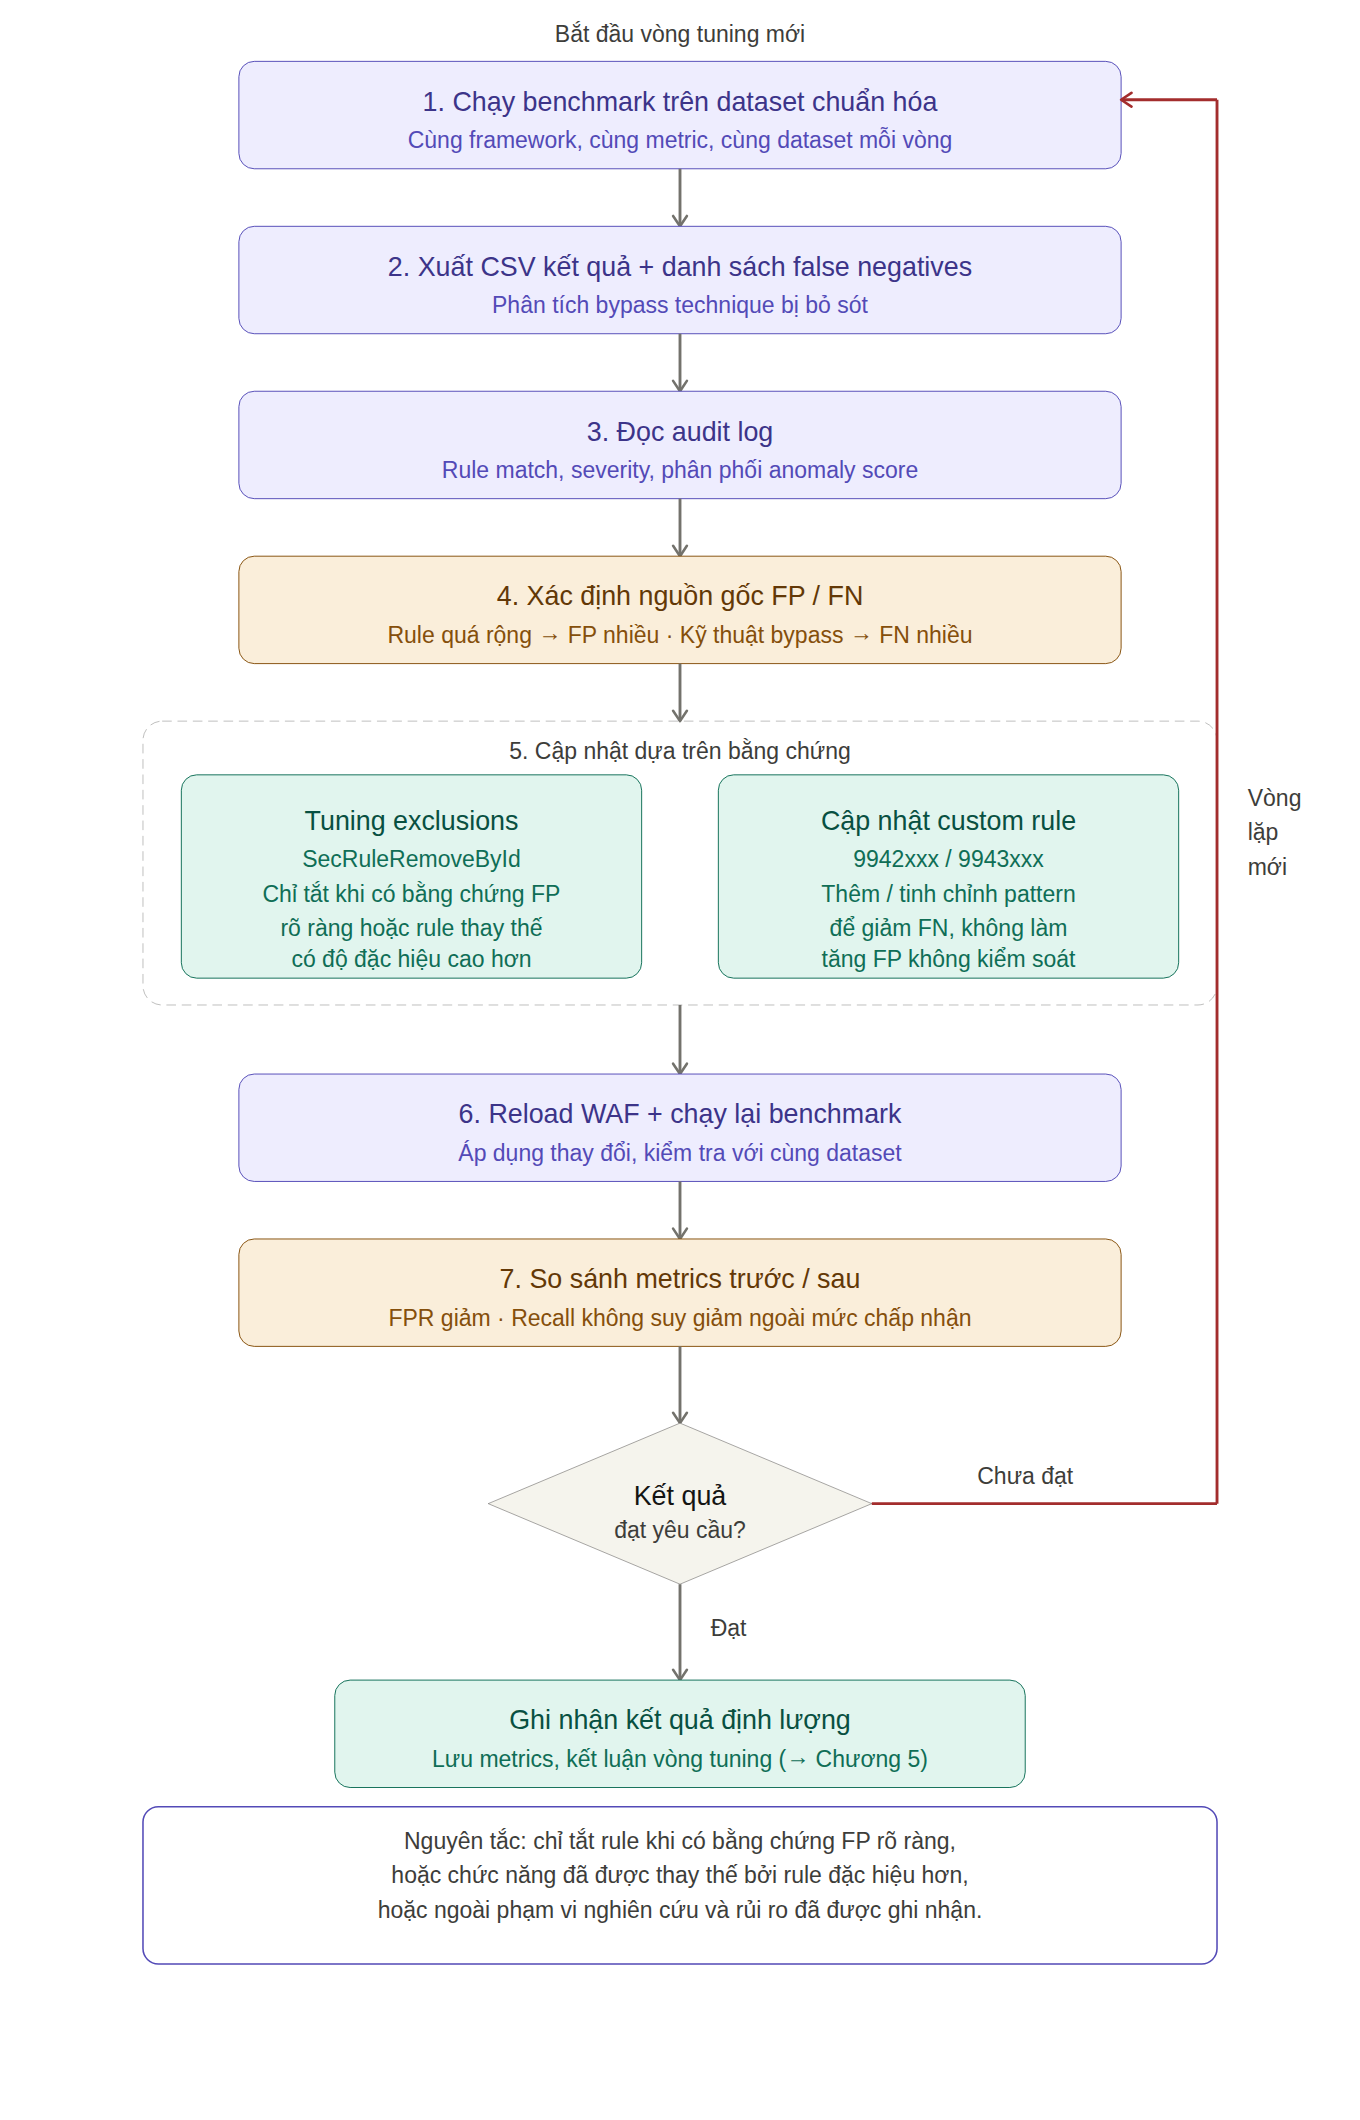
\includegraphics[width=0.92\textwidth,height=0.80\textheight,keepaspectratio]{Chapter3/tuning_iterative_process.png}
    \caption{Quy trình tuning exclusions và cập nhật rule dựa trên dữ liệu}
    \label{fig:tuning-iterative-process}
\end{figure}

Quy trình tuning gồm các bước sau:

\begin{enumerate}
    \item Chạy benchmark trên một hoặc nhiều dataset đã chuẩn hóa.
    \item Xuất CSV kết quả và danh sách false negatives để phân tích bypass.
    \item Đọc audit log để xác định rule match, severity và phân phối anomaly score.
    \item Xác định rule gây FP nhiều hoặc nhóm kỹ thuật gây FN nhiều.
    \item Cập nhật custom rule hoặc tuning exclusions dựa trên bằng chứng.
    \item Reload môi trường WAF và chạy lại benchmark.
    \item So sánh metrics trước/sau để bảo đảm FPR giảm mà recall không suy giảm ngoài mức chấp nhận.
\end{enumerate}

Chiến lược tuning không phải là tắt CRS một cách tùy tiện. Các custom rules v2 vẫn được giữ lại; CRS scoring engine vẫn được dùng để tổng hợp điểm; chỉ một số rule phát hiện gây nhiễu được loại khỏi pipeline. Với XSS, nhiều rule CRS nhóm \path|941xxx| được loại vì logic phát hiện đã được thay thế bằng XSS v2 có context rõ hơn. Với SQLi, một số rule \path|942xxx| được loại do quá nhạy hoặc trùng với semantic SQLi rules. Ngoài ra, một số rule protocol/character và RCE/Shell cũng được loại trong môi trường benchmark vì chúng nằm ngoài phạm vi chính XSS/SQLi hoặc tạo FP trên ký tự hợp lệ.

Bảng~\ref{tab:tuning-exclusions-groups} tóm tắt các nhóm exclusions quan trọng.

{\small
\renewcommand{\arraystretch}{1.2}
\begin{longtable}{|L{0.20\textwidth}|L{0.22\textwidth}|L{0.30\textwidth}|L{0.18\textwidth}|}
\caption{Các nhóm rule được tuning bằng SecRuleRemoveById}\label{tab:tuning-exclusions-groups}\\
\hline
\textbf{Nhóm rule} & \textbf{Ví dụ ID} & \textbf{Lý do thiết kế} & \textbf{Rủi ro/ghi chú} \\
\hline
\endfirsthead

\hline
\textbf{Nhóm rule} & \textbf{Ví dụ ID} & \textbf{Lý do thiết kế} & \textbf{Rủi ro/ghi chú} \\
\hline
\endhead

XSS CRS & \path|941100|, \path|941160|, \path|941390| & Giảm FP từ các rule XSS tổng quát, tránh trùng logic với XSS v2. & Cần bảo đảm XSS v2 cover đủ nhóm tấn công trong phạm vi. \\
\hline
SQLi CRS & \path|942100|, \path|942131|, \path|942370| & Giảm FP từ libinjection, character anomaly và rule SQLi quá rộng. & Tắt \path|942100| là trade-off vì mất một heuristic rộng. \\
\hline
Protocol/character & \path|920230|, \path|920272|, \path|920273| & Một số rule quá nghiêm với traffic benchmark hoặc input encoded hợp lệ. & Cần đánh giá lại nếu triển khai production. \\
\hline
RCE/Shell & \path|932120|, \path|932130|, \path|932231| & Giảm FP trên ký tự shell-like và nội dung ngoài phạm vi XSS/SQLi. & Rủi ro trung bình vì giảm coverage ngoài phạm vi đề tài. \\
\hline
Nhóm khác & \path|933161|, \path|934101| và một số rule lẻ & Loại bỏ các nguồn FP phát hiện qua audit log và benchmark. & Cần ghi nhận lý do tuning theo từng môi trường. \\
\hline
\end{longtable}
}

Cần nhấn mạnh rằng tuning exclusions là cấu hình phục vụ nghiên cứu và benchmark cho phạm vi XSS/SQLi. Nếu áp dụng trong production, người vận hành cần đánh giá lại theo traffic thật, loại ứng dụng, rủi ro cần bảo vệ và yêu cầu compliance. Đặc biệt, nhóm RCE/Shell và một số heuristic rộng của CRS không nên bị tắt mặc định nếu hệ thống cần bảo vệ toàn diện hơn ngoài XSS và SQLi.

Phần thiết kế tuning này là cơ sở kỹ thuật để trả lời RQ4 ở chương đánh giá. Kết luận về tuning không thể chỉ dựa trên việc số FP giảm, mà phải kiểm tra đồng thời FPR, recall và nhóm rule bị vô hiệu hóa để thấy rõ trade-off bảo mật.

\section{Khả năng bảo trì và giới hạn của giải pháp}
\label{sec:solution-maintainability-limitations}

Một hạn chế lớn của rule enumeration-based là regex dễ trở nên dài, khó đọc và khó kiểm thử khi danh sách payload tăng lên. Giải pháp v2 khắc phục bằng cách tổ chức rule theo namespace và layer rõ ràng. Dải \path|9942xxx| được dành cho XSS, dải \path|9943xxx| được dành cho SQLi. Trong mỗi dải, các rule được nhóm theo kỹ thuật: core, structural, encoded, DOM, advanced đối với XSS; classic, blind, error/OOB, advanced và heuristic đối với SQLi.

Cách tổ chức này giúp quá trình bảo trì có quy trình rõ hơn. Khi xuất hiện một bypass mới, người phát triển không cần thêm payload vào một regex lớn. Thay vào đó, có thể phân loại bypass thuộc nhóm nào: encoding, DOM context, protocol URI, time-based blind, comment obfuscation hay schema enumeration. Sau đó rule mới được thêm vào lớp tương ứng hoặc rule hiện có được chỉnh sửa có kiểm soát. Việc benchmark lại sau thay đổi giúp kiểm tra tác động tới cả recall và FPR.

Message, tag, severity và rule ID cũng hỗ trợ phân tích audit log. Khi request bị chặn, người vận hành có thể biết rule nào khớp, thuộc lớp nào, severity bao nhiêu và đóng góp điểm như thế nào vào anomaly score. Điều này giúp giải pháp dễ giải thích hơn so với mô hình AI black-box hoặc regex monolithic không có phân tách kỹ thuật rõ ràng.

Tuy nhiên, giải pháp vẫn có giới hạn. Custom rules v2 không thay thế hoàn toàn OWASP CRS, không tuyên bố phát hiện mọi biến thể XSS/SQLi trong tương lai và có thể vẫn tạo false positives trong các ứng dụng hợp lệ có chứa HTML, JavaScript hoặc SQL snippets. Base64 decode cũng cần được áp dụng cẩn trọng vì nhiều ứng dụng hợp lệ có thể truyền dữ liệu Base64 như ảnh, token hoặc blob dữ liệu. Cuối cùng, tuning exclusions trong môi trường benchmark không phải cấu hình production mặc định; các exclusions cần được xem xét lại theo yêu cầu bảo vệ của hệ thống thực tế.

Các nguyên tắc bảo trì này liên hệ trực tiếp với RQ1 và RQ3: nếu rule được tổ chức theo execution context và semantic pattern, việc mở rộng coverage không cần quay lại cách liệt kê payload đơn lẻ. Chúng cũng tạo cơ sở để thảo luận RQ5, vì khả năng giải thích bằng rule ID, message và severity là một ưu điểm quan trọng của WAF rule-based so với mô hình AI black-box.

\section{Tổng kết chương}
\label{sec:chapter3-summary}

Chương này đã trình bày phương pháp nghiên cứu và giải pháp đề xuất cho bài toán tối ưu bộ luật WAF. Quy trình nghiên cứu được tổ chức theo hướng lặp, bắt đầu từ phân tích CRS/rule gốc, thiết kế generalized rules, phân tích FN/FP và tuning dựa trên dữ liệu. Giải pháp được xây dựng trên ModSecurity/OWASP CRS, bổ sung hai nhóm custom generalized rules v2: XSS trong dải \path|9942xxx| và SQLi trong dải \path|9943xxx|.

Chương cũng đã trình bày decode pipeline trong luật phát hiện, cách rule v2 tích hợp với anomaly scoring của CRS, chiến lược tuning exclusions, khả năng bảo trì và các giới hạn của giải pháp. Chương tiếp theo sẽ trình bày thiết kế thực nghiệm và phương pháp đánh giá dùng để kiểm chứng các thành phần giải pháp vừa nêu.

\chapter{Giải pháp}
\label{chap:solution}

\section{XSS Rules v2}
\label{sec:xss-rules-v2}

Kiến trúc 5-Layer Defense với 30+ rules.

\section{SQLi Rules v2}
\label{sec:sqli-rules-v2}

Semantic-based detection với 14 rules.

\section{TUNNING-EXCLUSIONS.conf}
\label{sec:tuning-exclusions}

Cấu hình tắt 70+ CRS rules gây FP.

\chapter{Kết quả thực nghiệm và đánh giá}
\label{chap:results}

\section{Kịch bản đánh giá và liên kết với câu hỏi nghiên cứu}
\label{sec:results-evaluation-scenarios}

\subsection{Các cấu hình được so sánh}
\label{subsec:results-comparison-configurations}

\subsection{Ma trận câu hỏi nghiên cứu, dữ liệu và chỉ số đánh giá}
\label{subsec:results-rq-dataset-metrics}

\subsection{Nguyên tắc diễn giải kết quả}
\label{subsec:results-interpretation-principles}

\section{RQ1 -- Đánh giá khả năng giảm false positives của context-aware XSS rules}
\label{sec:rq1-context-aware-xss-fp}

\subsection{Kết quả trên Mereani clean}
\label{subsec:rq1-mereani-clean-results}

\subsection{Kết quả trên XSSed-DMOZ clean}
\label{subsec:rq1-xssed-dmoz-clean-results}

\subsection{Phân tích nguyên nhân giảm false positives}
\label{subsec:rq1-fp-reduction-analysis}

\subsection{Kết luận cho RQ1}
\label{subsec:rq1-conclusion}

\section{RQ2 -- Đánh giá multi-decode pipeline với payload encoded và obfuscated}
\label{sec:rq2-decode-pipeline-results}

\subsection{Kết quả trên GoTestWAF}
\label{subsec:rq2-gotestwaf-results}

\subsection{Coverage theo nhóm encoding và obfuscation}
\label{subsec:rq2-technique-coverage}

\subsection{Phân tích false negatives còn lại}
\label{subsec:rq2-false-negatives-analysis}

\subsection{Kết luận cho RQ2}
\label{subsec:rq2-conclusion}

\section{RQ3 -- Đánh giá coverage của semantic-based SQLi rules}
\label{sec:rq3-semantic-sqli-coverage}

\subsection{Coverage theo nhóm kỹ thuật SQL Injection}
\label{subsec:rq3-sqli-technique-coverage}

\subsection{So sánh với rule SQLi enumeration-based}
\label{subsec:rq3-enumeration-comparison}

\subsection{Phân tích false negatives SQLi}
\label{subsec:rq3-sqli-false-negatives}

\subsection{Kết luận cho RQ3}
\label{subsec:rq3-conclusion}

\section{RQ4 -- Đánh giá tác động của tuning exclusions}
\label{sec:rq4-tuning-exclusions-impact}

\subsection{So sánh trước và sau tuning}
\label{subsec:rq4-before-after-tuning}

\subsection{Phân tích các nhóm rule gây false positives}
\label{subsec:rq4-fp-rule-groups}

\subsection{Trade-off giữa FPR và recall}
\label{subsec:rq4-fpr-recall-tradeoff}

\subsection{Kết luận cho RQ4}
\label{subsec:rq4-conclusion}

\section{RQ5 -- So sánh với AI-based detection}
\label{sec:rq5-ai-based-comparison}

\subsection{Kết quả AI tham chiếu từ tài liệu}
\label{subsec:rq5-ai-reference-results}

\subsection{Hiệu năng thực nghiệm của WAF rule-based}
\label{subsec:rq5-waf-performance-results}

\subsection{So sánh về khả năng giải thích và vận hành}
\label{subsec:rq5-interpretability-operation-comparison}

\subsection{So sánh về độ trễ, cập nhật và triển khai real-time}
\label{subsec:rq5-latency-update-deployment-comparison}

\subsection{Kết luận cho RQ5}
\label{subsec:rq5-conclusion}

\section{Tổng hợp kết quả theo câu hỏi nghiên cứu}
\label{sec:results-summary-by-rq}

\subsection{Bảng tổng hợp kết luận theo RQ}
\label{subsec:summary-rq-conclusions}

\subsection{Các phát hiện chính}
\label{subsec:summary-main-findings}

\subsection{Chuyển tiếp sang chương thảo luận}
\label{subsec:summary-transition-to-discussion}

\chapter{Thảo luận và kết luận}
\label{chap:discussion-conclusion}

\section{Thảo luận}
\label{sec:discussion}

Phân tích rủi ro, so sánh với AI.

\section{Kết luận}
\label{sec:conclusion}

Đóng góp, giới hạn, hướng phát triển.



%--------------------------------------------- 
% References
%---------------------------------------------
% \bibliographystyle{IEEEtranSN}
\bibliographystyle{unsrt}
% % \renewcommand\bibname{Danh mục tài liệu tham khảo}
%\addcontentsline{toc}{chapter}{References}
\renewcommand\bibname{Tài liệu tham khảo}
\bibliography{references} % Path to your references.bib file

%--------------------------------------------- 
% Appendix
%---------------------------------------------
% \appendix
% \unchapter{Phụ lục}
\appendix

% \includepdf[pages=1,offset=0 0, pagecommand={\label{appendix}\thispagestyle{plain}}
% ]{Appendix/The-use-of-eye-tracking-in-supporting-individuals-with-dyslexia-a-review.pdf}





\end{document}
